%% 
%% Copyright 2007, 2008, 2009 Elsevier Ltd
%% 
%% This file is part of the 'Elsarticle Bundle'.
%% ---------------------------------------------
%% 
%% It may be distributed under the conditions of the LaTeX Project Public
%% License, either version 1.2 of this license or (at your option) any
%% later version.  The latest version of this license is in
%%    http://www.latex-project.org/lppl.txt
%% and version 1.2 or later is part of all distributions of LaTeX
%% version 1999/12/01 or later.
%% 
%% The list of all files belonging to the 'Elsarticle Bundle' is
%% given in the file `manifest.txt'.
%% 
%% Template article for Elsevier's document class `elsarticle'
%% with harvard style bibliographic references
%% SP 2008/03/01

\documentclass[final,3p,times,twocolumn]{elsarticle}

%% Use the option review to obtain double line spacing
%% \documentclass[authoryear,preprint,review,12pt]{elsarticle}

%% Use the options 1p,twocolumn; 3p; 3p,twocolumn; 5p; or 5p,twocolumn
%% for a journal layout:
%% \documentclass[final,1p,times,authoryear]{elsarticle}
%% \documentclass[final,1p,times,twocolumn,authoryear]{elsarticle}
%% \documentclass[final,3p,times,authoryear]{elsarticle}
%% \documentclass[final,3p,times,twocolumn,authoryear]{elsarticle}
%% \documentclass[final,5p,times,authoryear]{elsarticle}
%% \documentclass[final,5p,times,twocolumn,authoryear]{elsarticle}

%% For including figures, graphicx.sty has been loaded in
%% elsarticle.cls. If you prefer to use the old commands
%% please give \usepackage{epsfig}
%\usepackage{ecrc}

%% The amssymb package provides various useful mathematical symbols
\usepackage{amssymb}
%% The amsthm package provides extended theorem environments
\usepackage{amsthm}
\usepackage{mathtools}
\usepackage{hyperref}	
\usepackage{lipsum}% http://ctan.org/pkg/lipsum
\usepackage{graphicx,subfigure}
\usepackage{tikz}
\usetikzlibrary{shapes,snakes}

\usepackage[ruled,vlined,linesnumbered,boxed]{algorithm2e}
\usepackage{color}

\usepackage{cancel}
\usepackage{placeins}
\newcommand\Ccancel[2][black]{\renewcommand\CancelColor{\color{#1}}\cancel{#2}}
\usepackage{tcolorbox}


%% The lineno packages adds line numbers. Start line numbering with
%% \begin{linenumbers}, end it with \end{linenumbers}. Or switch it on
%% for the whole article with \linenumbers.
%%\usepackage{lineno}
\usepackage{xcolor}
\usepackage{blindtext}
\definecolor{red}{rgb}{1,0,0}
\newcommand{\red}[1]{\textcolor{red}{#1}}

%\newcommand{\X}{\mathbf{x}}
%\newcommand{\B}{\mathbf{b}}
%\newcommand{\U}{\mathbf{u}}
\newcommand{\X}{x}
\newcommand{\B}{b}
\newcommand{\U}{\dot{x}}

%\newcommand{\Ui}{\mathbf{u}^{[i]}}
%\newcommand{\Bi}{\mathbf{b}^{[i]}}
%\newcommand{\Xm}{\mathbf{x}^{[m]}}

\newcommand{\Ui}{\dot{x}^{[i]}}
\newcommand{\Bi}{b^{[i]}}
\newcommand{\Xm}{x^{[m]}}

\newcommand{\invSigK}{\boldsymbol{\Sigma}^{[k]^{-1}}}
\newcommand{\SigK}{\boldsymbol{\Sigma}^{[k]}}
\newcommand{\Sig}[1]{\boldsymbol{\Sigma}^{[#1]}}
\newcommand{\Mu}[1]{\boldsymbol{\mu}^{[#1]}}
\newcommand{\MuK}{\boldsymbol{\mu}^{[k]}}
\newcommand{\xb}{\dot{x}|b}

\newcommand{\piK}{w^{[k]}}
\newcommand{\Param}{\boldsymbol{\theta}}
\DeclareMathOperator*{\argmax}{arg\,max}

\makeatletter
\newcommand{\removelatexerror}{\let\@latex@error\@gobble}
\makeatother

\graphicspath{ {Figures/}{Figures/Results1} }

\journal{Robotics and Autonomous Systems}

\begin{document}

\begin{frontmatter}

%% Title, authors and addresses

%% use the tnoteref command within \title for footnotes;
%% use the tnotetext command for theassociated footnote;
%% use the fnref command within \author or \address for footnotes;
%% use the fntext command for theassociated footnote;
%% use the corref command within \author for corresponding author footnotes;
%% use the cortext command for theassociated footnote;
%% use the ead command for the email address,
%% and the form \ead[url] for the home page:
%% \title{Title\tnoteref{label1}}
%% \tnotetext[label1]{}
%% \author{Name\corref{cor1}\fnref{label2}}
%% \ead{email address}
%% \ead[url]{home page}
%% \fntext[label2]{}
%% \cortext[cor1]{}
%% \address{Address\fnref{label3}}
%% \fntext[label3]{}

\title{Fitted Policy Iteration for a POMDP Peg-In-Hole search task.}

%% use optional labels to link authors explicitly to addresses:
%% \author[label1,label2]{}
%% \address[label1]{}
%% \address[label2]{}

\author{Guillaume de Chambrier, Aude Billard}

\address{}

% A  concise  and  factual  abstract  is  required.  The  abstract  should  state  briefly  the  purpose  of  the
% research, the principal results and major conclusions. An abstract is often presented separately from
% the article, so it must be able to stand alone. For this reason, References should be avoided, but if
% essential, then cite the author(s) and year(s). Also, non-standard or uncommon abbreviations should
% be avoided, but if essential they must be defined at their first mention in the abstract itself


%We consider two types of explanatory 
%tasks for which the correct handling of uncertainty is necessary; The first is the peg-in-hole insertion task
%which is widely present in manufacturing assembly processes, which requires a high level of 
%precision on the millimetre scale. The second is search, such as looking for a patient in a hospital or finding 
%people in search and rescue operations.
%.

\begin{abstract}

% Introduce the Problem
%Acting optimally given environmental uncertainty is still currently a major concern for autonomous robotic 
%systems. Uncertainty arises from the absence of informative prior knowledge, insufficient sensor capabilities 
%and imprecise motion. Such uncertainty, if not considered appropriately by a policy or planner can lead 
%to either sub-optimal task execution or failure. We consider a plug power-socket search and connection task 
%also known as Peg-in-Hole (PiH) in which both a human and robot must be able to find a socket and connect a power 
%plug to it without using any vision, making the state space partially observable, whilst solely relaying on haptic information.

A policy can be obtained by encoding the tasks as a partially observable markov decision process (POMDP) and 
then solve it by dynamic programming. This quickly become infeasible for relatively high-dimensional continuous tasks.  
To address this problem we demonstrate how human intuition can be leveraged to learn a belief space policy. A set 
of human teachers demonstrate the search PiH task during which the position uncertainty, represented by a Point Mass Filter (PMF),
is recorded and compressed to the most likely state and entropy. 
A policy parametrised by a Gaussian Mixture Model (GMM) is learned and refined in an Actor-Critic Fitted reinforcement learning framework.
We evaluate Actor-Critic policy, called Q-EM, against a Greedy and non-optimised GMM policy with respect to the distance taken to localise the socket
and the distance taken to establish a connection between the plug and power socket. We test the ability of the learned models 
to generalise to different socket types and locations. We found that the Actor-Critic policy is always better in terms of 
distance travelled to localise the socket. We tested on a KUKA LWR robot, across three different power sockets, the ability of 
the Q-EM, GMM and Greedy policies to find and connect a plug to the power socket.
We found when the socket has no distinctive features both data learned policy are better but when features are present the 
Greedy policy does just as good, or better.

%We evaluate the learned policy in three ways; We first compare our policy against a greedy one. Secondly we compare the 
%effect of using reinforcement learning against a purely statistical controller. Thirdly we evaluate the importance of 
%the provided human demonstrations, the data.
\end{abstract}

\begin{keyword} 
Programming by Demonstration, Actor-Critic, Belief Space, POMDP, Fitted Reinforcement Learning
\end{keyword}

\end{frontmatter}

% State the objectives of the work and provide an adequate background, avoiding a detailed literature
% survey or a summary of the results.
% - Establish context of work being reported (POMDP, learning search behaviour, etc..), discuss primary 
%   relevant research literature
% - State the Purpose of the work in the form of hypothesis, question, or problem you investigate; and,
%
%    Quite literally, the Introduction must answer the questions, "What was I studying? Why was it an important question? 
%    What did we know about it before I did this study? How will this study advance our knowledge?"
%
% - Structure: inverse pyramide, Start very general and then narrow down. Finally arrive at statement, purpose of rational.
%
% 1) Clearly identifying the subject area.

% Background
% 2) Establishing the context by providing a brief and balanced review of the pertinent published 
%    literature that is available on the subject.
% -> say what we knew before doing this problem. 

% 3) Be sure to clearly state the purpose and / or hypothesis that you investigate

\section{Introduction}

The ability to act optimally given uncertainty is paramount for robotic systems to be successful in
environments which are not fully observable. Depending on the task and structure of the uncertainty, 
if not taken into consideration by the control policy, can lead to waist-full usage of resources 
and even fail to accomplish the task. interinerin

An approach is to formulate the task as partially observable markov decision process (POMDP) which is subsequently
solved by dynamic programming. It is well known that solving a POMDP directly is infeasible even for 
the simplest problems[cite]. In this work we introduce a Fitted Policy Iteration Actor-Critic 
Reinforcement Learning (RL) method in which sample episodes are provided by human teachers in 
a Programming by Demonstration (PbD) framework. We consider a plug power-socket search and connection 
task (also known as Peg-in-Hole (PiH)) in which a robot apprentice must learn how to localise a 
power socket and then establish a connection. 
No vision system is used during the task and we will solely relay on haptic information, provided via force-torque sensor mounted on the end-effector 
of the robot. We chose to not use vision for two reasons. The first is that we want to 
know the humans capabilities of accomplishing the task under these conditions and whether 
we can learn a POMDP policy from their demonstrations. The second is that PiH is a very important 
component in manufacturing processes and we seek to demonstrate that we accomplish the task without 
the need of a vision system which would result in additional costs.

The rest of the paper is organised as follows: Section \ref{sec:related_work} overic, 
Section \ref{sec:experiment_methods}, Section \ref{sec:learning-value-actor}, 
Section \ref{sec:FPI}, Section \ref{ch4:control_architecture}, Section \ref{sec:results}, Section \ref{sec:conclusion}


\section{Related work}\label{sec:related_work}

There are two research domains which are closely related to our work. The first 
is Fitted Reinforcement learning (also know as Batch or Experience replay) and the 
second is Peg-in-hole.

\subsection{Peg-in-hole}

The Peg-in-Hole (PiH) task is one of the most widespread step in industrial assembly and manipulations processes, 
with examples including the assembly of vehicular transmission components \cite{search_strategies_icra_2001} and 
valves \cite{online_gpr_icra_2014}. To be successful, the estimated position of the robot's end-effector 
and workpiece must be precise. Typically, the clearance between peg and plug is very small leaving little 
room for error.

All approaches use to some extent a vision system \cite{peg_personal_icra_2010} to estimate 
the position of the workpiece. Given  the peg's estimated position with respect to the hole 
an insertion strategy has to be carried since the hole will be occluded by 
the robot's manipulator. One approach is to apply blind search patters, such as circular 
motions \cite{search_strategies_icra_2001}, which do not consider actual state uncertainty. 
These approaches work well when the plug or peg is within the vicinity. In our work we consider 
no visual information which leads to high state uncertainty making the direct application 
of such blind search methods ill-suited.

Another approach consists of learning task space policies and gradually adapt its parameters based on a reference
Force/Torque profile. In \cite{fast_peg_pbd_icmc_2014} the authors learned a time-dependent Dynamic Movement 
Primitive (DMP) \cite{Schaal04learningmovement} Cartesian end-effector policy for the Cranfield benchmark 
object from human teleoperated demonstrations. Similarly in \cite{trans_workpiece_icra_2013,sol_pdg_pbd_2014}, 
a F/T profile is encoded separately by a regressor function along the DMP policy. Successive refinements of 
the DMP policy are achieved through using force feedback to adapt the parameters of an admittance controller such 
to reproduce the same F/T (encoded by a separate regressor).

Reproducing exactly the same force torque profile for the full trajectory which is encoded in a time dependent dynamical system might be 
unnecessary as the force torque profile is predominantly useful during the final stage of the PiH task, 
where the insertion can cause jamming. The force torque information can be used to rectify 
this problem \cite[Chap. 5]{Kronander2015}. 

% RL
Reinforcement learning has also been applied to PiH. In \cite{learn_force_c_icirs_2011} a DMP policy is 
initialised with kinesthetic demonstrations of picking up a pen. The recorded Cartesian 
trajectories are encoded in a parameterised DMP policy and augmented with a F/T profile. 
After 110 trials the policy was found to be a 100\% successful. In \cite{learn_admittance_icra_1994} a 18 dimensional input 
and a 6 dimensional output (linear and angular velocity) neural network is learned. After a 100 episodes the policy 
was shown to be successful. Our work is similar in its approach, however we will not be considering autonomous rollouts 
common in RL, but will rely solely on the initial data provided by human teachers.

\subsection{Actor-Critic \& Fitted Reinforcement Learning}

Actor-critic \cite[Chap. 6.6]{sutton98a} (AC) use two separate parameterisation of the policy (actor) and 
value function (critic). It has been reported and proven \cite{rl_ac_surv_2012} to be faster than policy 
search methods as the variance in the gradient estimate is smaller. The advantage of an AC is that 
the policy can be chosen such that it is computationally efficient in evaluating actions and the 
value function does not necessarily have to have the same function representation and parameterisation 
as the actor.

To guarantee convergence (in model based RL) during temporal difference learning, 
the value function approximators has to be an averager (tile coding, k-nearest-neighbour, locally weighted averaging) 
\cite{stable_FA_gordon_1995}. The extension to a model-free approach with a kernel function approximator 
(locally weighted averaging, the kernel is a Gaussian function) known as Kernel-Based Approximate Dynamic Programming (KBDP) \cite{kernel_rl_ormoneit_2002}
has proven to be globally optimal in a continuous-space framework. This leads to the wider application of Batch RL methods 
such as Fitted Value Iteration (FVI) \cite{fvi_uav_2010} and Fitted Q-Iteration (FQI) \cite{EGW05} (Q-approximator is a random forest ensemble),
\cite{fqi_nips_peter_2009} to the RL community. By remembering all the state transition pairs and by applying multiple 
synchronous Dynamic Programming (DP) and function approximation updates, the problem of diverging value function approximators is resolved. 

Retaining all the data makes it in practice easy to apply function approximators which are not averagers, such as neural networks,
to RL problems. A successful example was Neural Fitted Q-Iteration (NFQI) \cite{Riedmiller2005} which 
uses a multi-layer perceptron to represent the Q-function for the cart-pole and mountain car problems and 
shows rapid convergence to optimal policies. It has since been used in many extensions, \cite{NAC_2008}, \cite{rl_gmm_2010}.
This has lead to the application of more sophisticated regression methods such the increasingly popular Deep Learning methods 
which are known as Deep Fitted Q-iteration (DFQ) \cite{Lange_riedmiller_2010} (used to learn visual control policies) 
and with recent work including learning to play ATRI and ping-pong games \cite{mnih-dqn-2015}, \cite{DRQ_AAAI_2015}. 

The reader is referred to \cite{approx_rl_overview_2011} and \cite[Chap 2]{RL_state_art_2012} for a literature 
review which includes a taxonomy of Batch RL methods and to  for a concise description Batch RL beginning at 
its origins, how it became popular with Fitted RL approaches and its continuation into Deep Learning.

The Fitted Policy Iteration which we apply to our belief space PiH search task is part of this family of methods.
We chose an on-policy approach to avoid the maximisation over the actions, as we are in continuous action space.
We use a Gaussian Mixture Model to parameterise the policy and a Locally Weighted Regression (LWR) as 
the value function approximator.


\section{Experiment methods}\label{sec:experiment_methods}

Figure \ref{fig:search_task_setup} (\textit{Top-left}), illustrates the PiH-search experiment setup. The orange area represents 
the teachers starting area and is assumed prior knowledge. The sockets are always positioned at the center of a fake wall (wooden plank) which is clamped to a table, see 
Figure \ref{fig:search_task_setup} (\textit{Top-right}) for an illustration. 
We consider one type of plug, Type J\footnote{http://www.iec.ch/worldplugs/typeJ.htm}, and three different power sockets. 
Power \textit{socket A}, has a ring around its holes, \textit{socket B} has a funnel, which we hypothesize should make 
it easier to connect, and \textit{socket C} has a flat elevated surface. See Figure \ref{fig:search_task_setup}
(\textit{Bottom}) for an illustration. 

\begin{figure*}
 \centering
 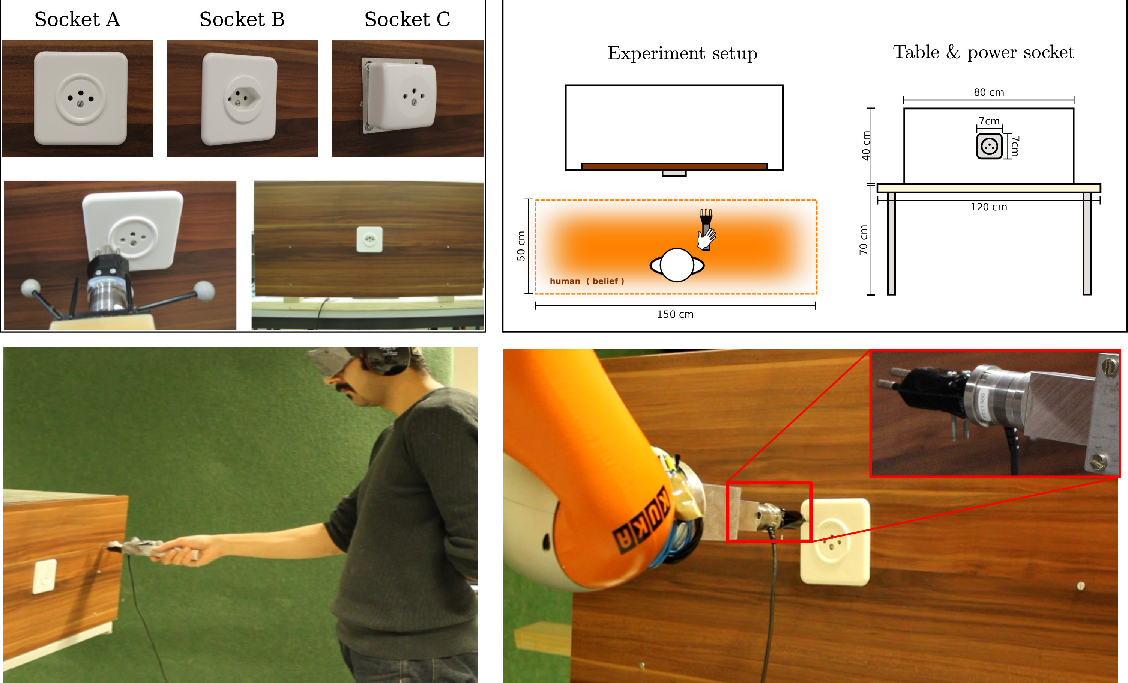
\includegraphics[width=0.8\textwidth]{./Figure/Figure1.pdf}
 \caption{The experimental setup. \textit{Top-left:} A participant (human teacher) is blindfolded and 
    placed within the orange rectangular area always facing the wall. \textit{Top-right:} Dimensions of the 
    the wall and socket. \textit{Bottom:} Three different power sockets, only socket A and B are used for data collection, socket
    C is purely used for evaluating the generalisation of the learned policy.}
    \label{fig:search_task_setup}
\end{figure*}

The human teacher holds the plug which is attached to a cylindrical handle with 
an ATI 6 axis force torque sensor (Nano25 \footnote{http://www.ati-ia.com/products/ft/sensors.aspx}) 
to provide \textbf{raw} wrench $\phi \in \mathbb{R}^6$ measurements. We define the \textbf{actual} measurement 
to be a function of the raw wrench, $\tilde{y}_t = h(\phi_t)$, which is a binary feature vector. The feature vector encodes whether a contact is present 
and the direction in which it occurs, which is discretized to the four cardinalities.

On top of the cylinder there is a set of markers used by a motion capture system 
OptiTrack\footnote{http://www.optitrack.com/} (which has millimeter tracking accuracy), 
see Figure \ref{fig:plug_cylinder}, to measure both linear, $\dot{x} \in \mathbb{R}^3$, 
and angular velocity, $\omega \in \mathbb{R}^3$, at each time step which is recorded at 
a rate of 100 Hz along with the F/T information.


The human's location belief is represented by a probability density function (pdf) which 
is assumed to be uniformly distributed in the orange area of Figure \ref{fig:search_task_setup}
and that all subsequent beliefs can be inferred from the measured velocity and measurements 
provided by the ATI and OptiTrack sensors.

\subsection{Belief state}

For the task at hand, the belief probability density function,  $p(x_t|y_{0:t},\dot{x}_{1:t})$,  
is a Point Mass Filter (PMF) \cite[p.87]{Bergman99recursivebayesian}, which is a non-parametric  Bayesian filter.
In Figure \ref{fig:PMF} (\textit{Bottom-right}) we illustrate the likelihood when an edge is sensed. 
A PMF is chosen to represent the believed location of the plug as the sensing likelihoods are non-gaussian and 
lead to multi-modal distributions. 

\begin{figure*}
 \centering
   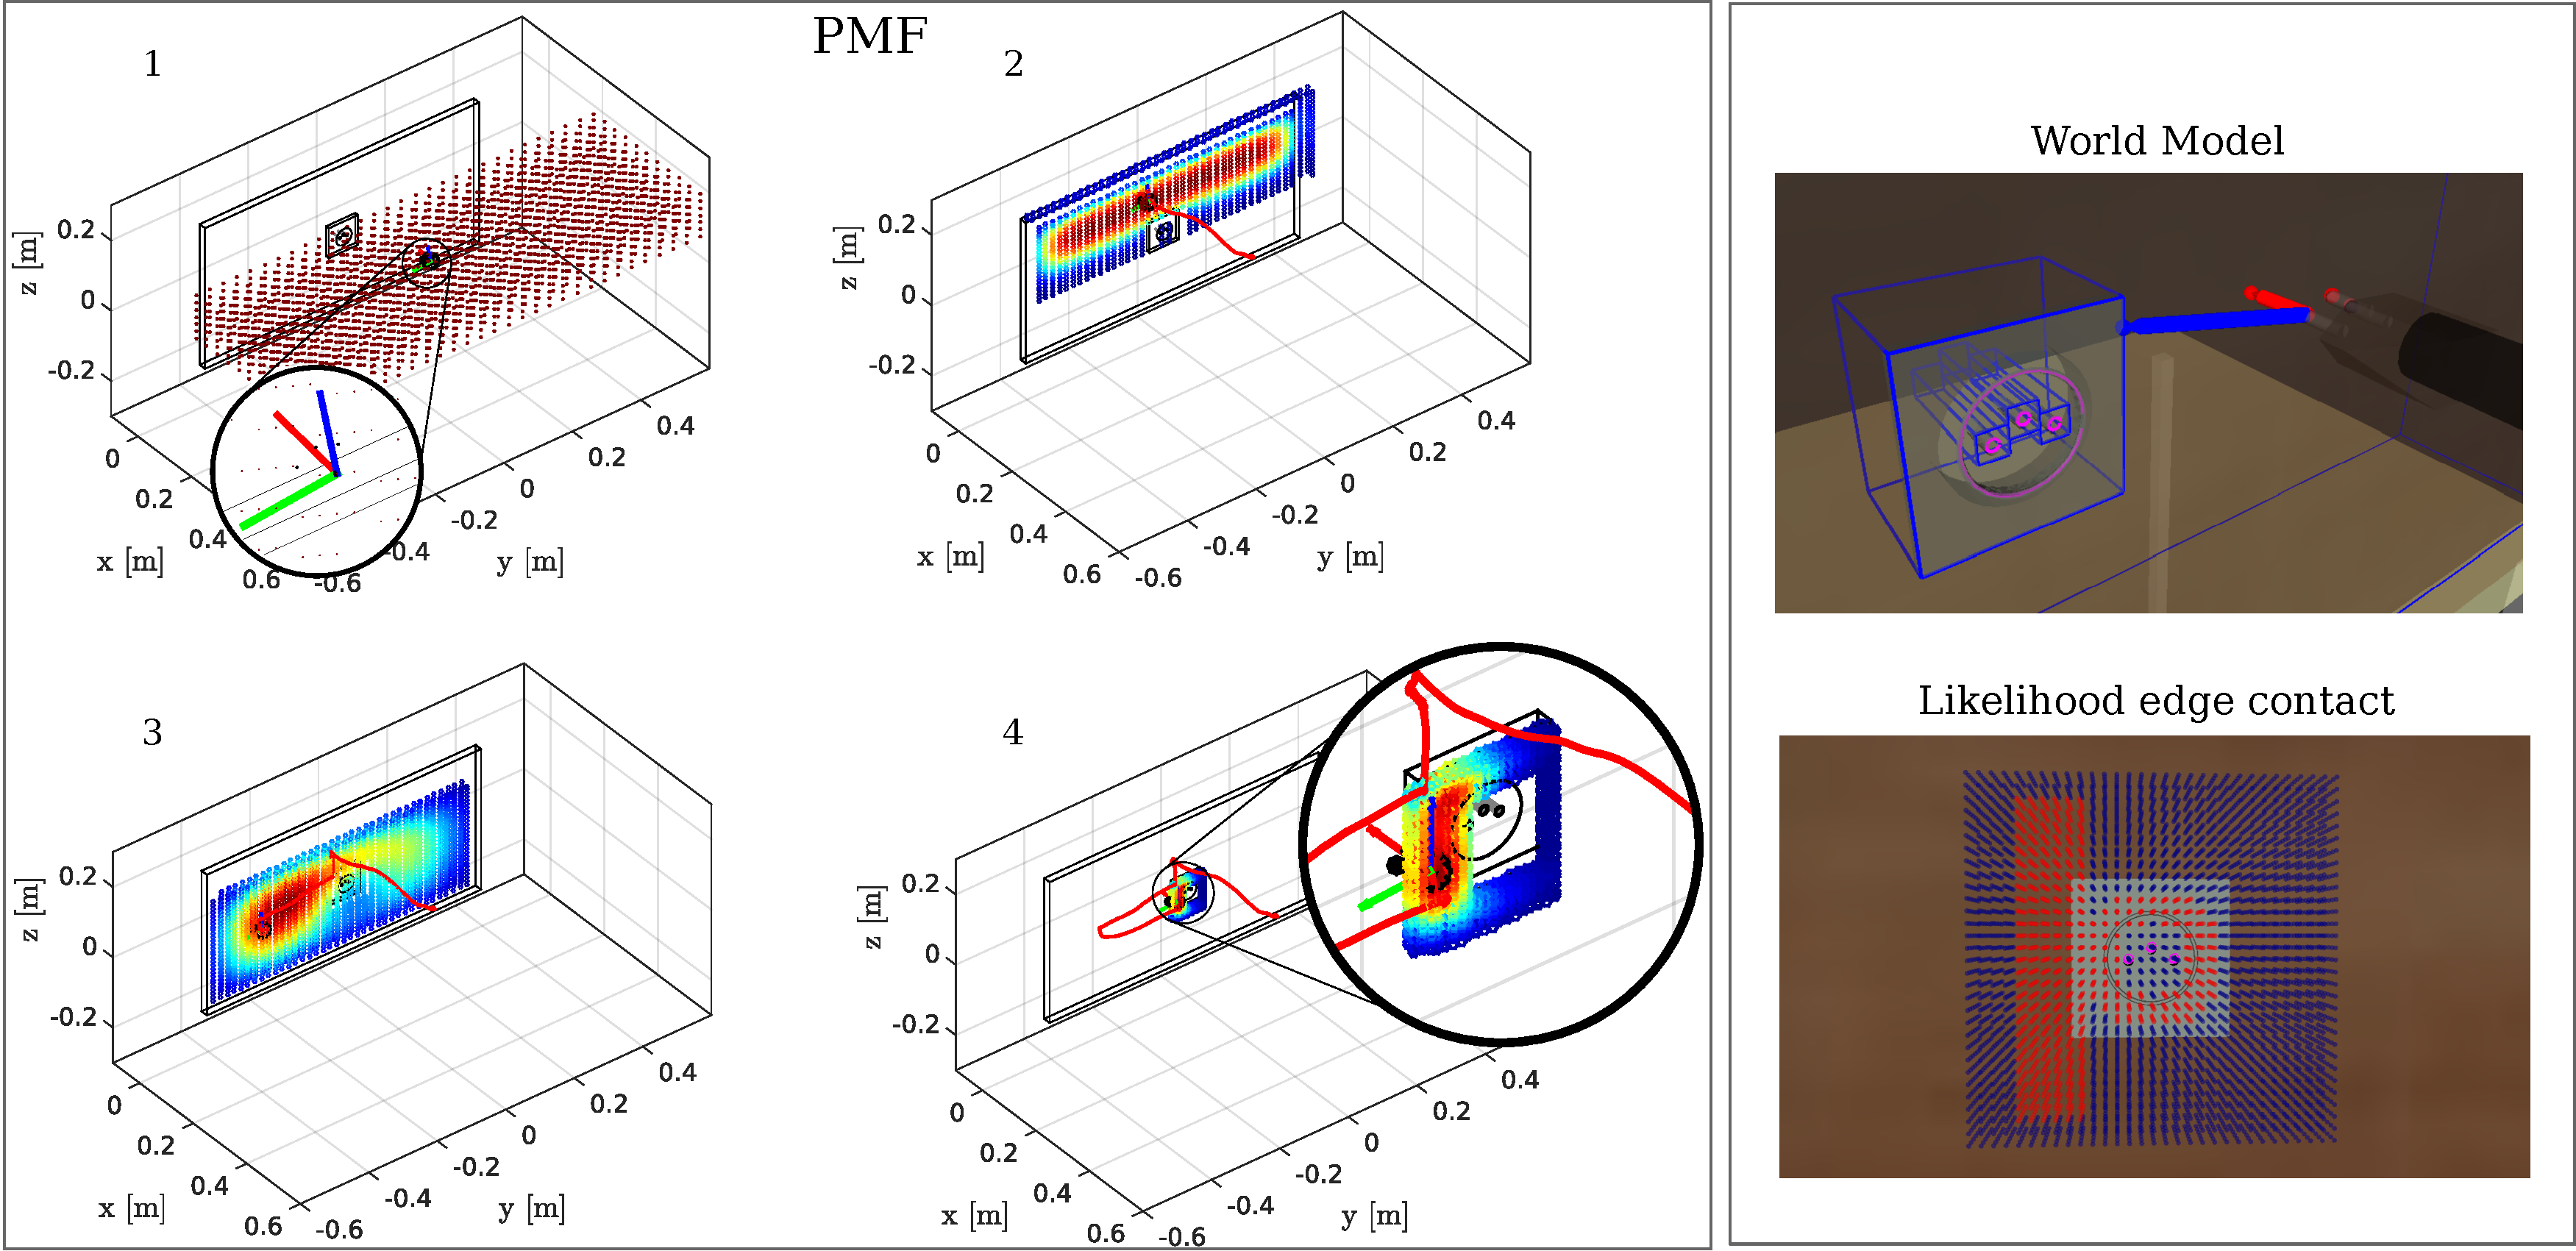
\includegraphics[width=0.95\textwidth]{./Figure/Figure2.pdf}
   \caption{\textit{Left:} Point Mass Filter (PMF) update of a particular human demonstration. (1) Initial uniform distribution spread over the starting 
   region. Each grid cell represents a hypothetical position of the plug. The orientation is assumed to be known. (2) First contact, the distribution 
   is spread across the surface of the wall. The red trace is the trajectory history. (3) motion noise increases the uncertainty. (4) The plug is in contact with a socket edge.
   \textit{Right}: \textbf{World model}: The plug is modelled by its three plug tips and the wall and sockets are fitted with bounding boxes.
   \textbf{Likelihood}: The plug enters in contact with the left edge of the socket. As a result, the value of the likelihood in all the regions, $x_t$, close the left edge take 
   a value of one (red points)  whilst the others have a value zero (blue points) and areas around the socket's central 
   ring have a value of one. }
  \label{fig:PMF}
\end{figure*}

The pdf is high dimensional and thus it is impractical to directly learn a statistical 
policy ${\pi_{\theta} : p(x_t|y_{0:t},\dot{x}_{0:t}) \rightarrow \dot{x}_t}$ without some form of compression. 
We compress it to a belief space vector $b_t = [\hat{x}_t,U]^{\mathrm{T}}$ composed of the maximum a posteriori, 
$\hat{x}_t \in \mathbb{R}^3$, and the differentiation entropy, $U = H\{p(x_t|y_{0:t},\dot{x}_{0:t})\} \in \mathbb{R}$.

Each participant's demonstration results in a dataset $D=\{\dot{x}^{[i]}_{1:T},\omega^{[i]}_{1:T},\phi^{[i]}_{1:T},b^{[i]}_{1:T}\}$, 
where the upper index $[i]$ references the ith search trajectory (also one execution of the task or one episode) and 
subscript $1:T$ denotes the time steps during the trajectory from initialisation $t=1$ until the end $t=T$. 

\subsection{Participants and experiment protocol}

To perform the PiH search tasks we recruited 10 student volunteers to be teachers (all male Master's and PhD students).
The participants were aged between 24 and 30 with an average age of 26 years and a standard deviation of 2.4 years.
Each participant carried out 30 demonstrations of the PiH search-task and each session lasted approximately 50 minutes and 
never exceeded one hour. The 10 participants were divided equally in two groups, A and B. Each member of group A began 
by performing 15 PiH searches with socket A, followed by a 10 minute break, finishing with an additional 15 searches with socket B. 
The members of group B performed the same protocol starting with socket B and ending with socket A.
Figure \ref{fig:experiment_design} summarises a walk through of the experiment.
The only exclusion criteria was the inability of the subject to accomplish the task. All participants gave written consent 
for taking part in this study. Each participant carried out a total of 30 PiH-search experiments, giving a 
total of 300 demonstrations
Both groups A and B took $9\pm10$s to find the socket's edge, regardless of the socket type. This is to be expected since the sockets 
are at the same location. It took a further $8\pm7$s on average for group B to connect
socket B and $12\pm10$s on average for group A to connect socket A. As we can see this is not a straight forward task when considering
the sensory deprivation. See Figure \ref{fig:experiment_setup_data} (\textit{Bottom}) for the time taken to connect the plug to the socket.

%In Appendix \ref{app:anova_socket} we report the results of a non-parametric statistical analysis on the time taken to connect
%the sockets and we find that it takes 4 seconds more to connect socket A than socket B. This is somewhat expected as 
%socket B has a funnel which can help to contain the subject to within the vicinity of the holes.
%As connecting to socket A is more difficult we will \textbf{using only these demonstrations} as training data to learn a policy. Both
%socket B and C will be used solely to evaluate the generalisation of the policy.


\begin{figure}
\centering
 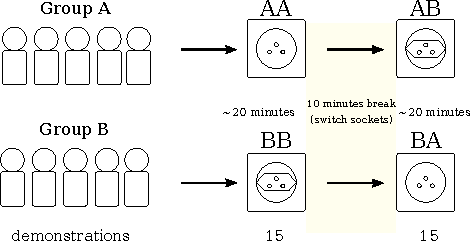
\includegraphics[width=0.9\linewidth]{./Figures/Fig/experiment_design_v2.pdf}
 \caption{Experiment protocol. The participants are divided in two groups of 5, Group A begins with socket A 
 and after a short break repeats the task with socket B. The same logic holds for Group B.
 For each socket 15 executions of the task are recorded.}
 \label{fig:experiment_design}
\end{figure}


\begin{figure}
 \centering
   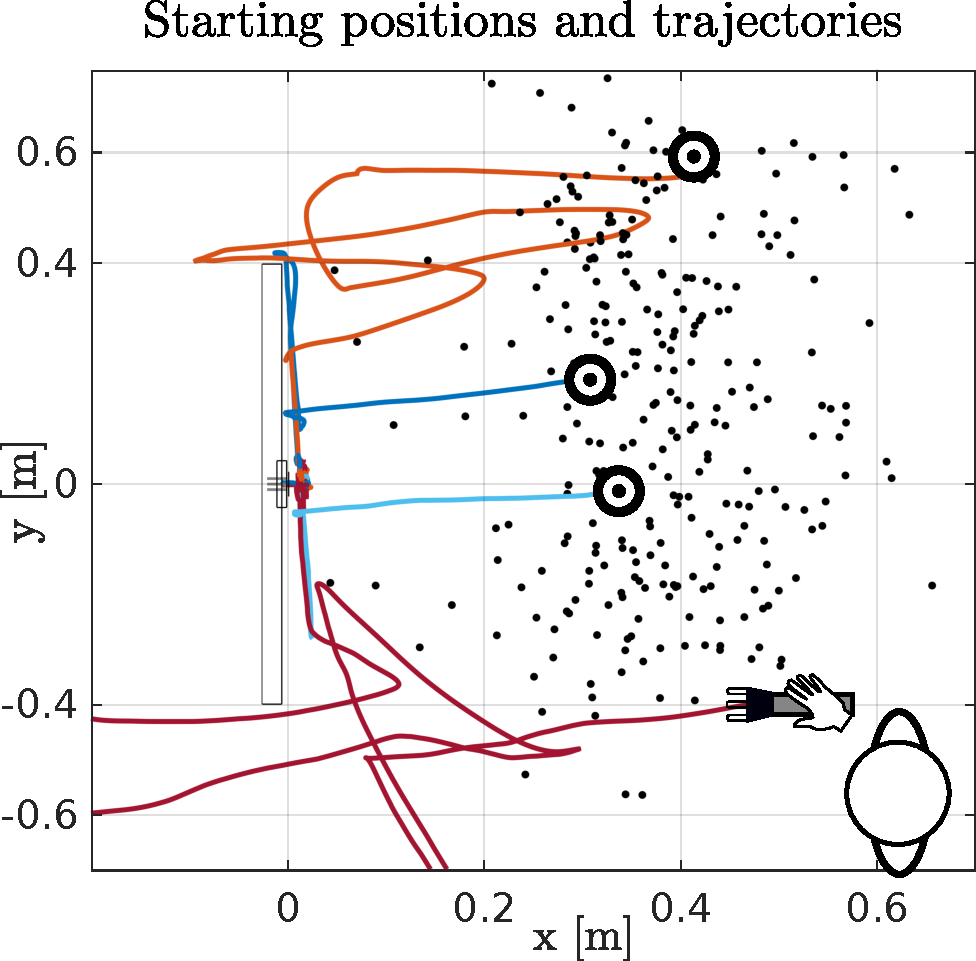
\includegraphics[width=0.9\linewidth]{./Figure/time_taken.pdf}
   \caption{\textit{Top}: Black points represent the starting position of the end-effector
   for all the demonstrations. Four trajectories are illustrated.}
  \label{fig:experiment_setup_data}
\end{figure}

\section{Learning Actor and Critic}\label{sec:learning-value-actor}

We learn two policies. The first policy maps from belief space 
to linear velocity $\pi_{\Param_1} : b_t \mapsto \dot{x}_t$ and the second from 
sensed wrench to angular velocity, $ \pi_{\Param_2} : \phi_t \mapsto \omega_t$.
The belief policy $\pi_{\Param_1}$ is learned in a Fitted Actor-Critic framework 
and the wrench policy $\pi_{\Param_2}$ directly from the demonstrated data as was done 
in \cite[Chap. 5]{Kronander2015}, which proved to be efficient in overcoming jamming during the PiH. 
Our objective is to maximise the parameters of the policy, $\pi_{\Param_1}: b \mapsto \dot{x}_t$, 
with respect to the value function:
\begin{equation}\label{eq:value_function}
  V^{\pi_{\Param_1}}(b_t) = \mathbb{E}_{\pi_{\Param_1}}\Bigg\{ \sum_{t=0}^{\infty} \gamma^{t} r_{t+1} | b_0=b,\pi_{\Param_1}\Bigg\}
\end{equation}
where $r_t \in \mathbb{R}$ is the reward and $\gamma \in [0,1)$ the discount factor. It is the expected future reward given the current 
belief state and policy. For our PiH-search task we assign a reward of $r=0$ at each time step until the goal
(plug-socket connection) is achieved, where a reward of 100 is given, $r_{T}=100$. Given the continuous nature and 
dimensionality of the belief space we use Locally Weighted Regression \cite{Atkeson97locallyweighted} (LWR) as a function 
approximator of the value function, $V^{\pi}(b)$.

 In an Actor-Critic setting, 
the temporal difference error, ${\delta^{\pi}_t = r_{t+1} + \gamma V^{\pi}(b_{t+1}) - V^{\pi}(b_t)}$, of the value 
function is used as a learning signal to update simultaneously itself and the actor (the policy).

\subsection{Actor \& Critic}
Both the linear and angular velocity policies are parameterised by a Gaussian Mixture Model (GMM), Equation \ref{eq:GMM}.

\begin{equation}
 \pi_{\Param_1}(\U,\B) = \sum\limits_{k=1}^{K} \piK \, g(\U,\B;\MuK,\SigK) \label{eq:GMM}
\end{equation}
The parameters $\Param = \{w^{[k]},\MuK,\SigK\}_{1,\dots,K}$, are the weights, means and covariances 
of the individual Gaussian functions, $g(.)$,
\begin{center}
$\MuK =  \begin{bmatrix} \MuK_{\U} \\ \MuK_{\B} \end{bmatrix}$, 
$\SigK =  \begin{bmatrix} 
	  \SigK_{\U\U} & \SigK_{\U\B} \\
	  \SigK_{\B\U} & \SigK_{\B\B}
	  \end{bmatrix}$
\end{center}
where $\sum_{k} w^{[k]} = 1$, $\MuK_{\U} \in \mathbb{R}^{3}$ and  $\MuK_{\B} \in \mathbb{R}^{4}$.
In both cases we use the Bayesian Information Criterion to determine the number of Gaussian functions.
In the next section, we will show how the parameters of $\pi_{\Param_1}$ can be adapted by the value function.


\subsection{Fitted Policy Iteration}\label{sec:FPI}

\paragraph{Policy evaluation}

To learn the value function we take Fitted RL \cite{EGW05} approch, 
This is an offline method which applies multiple sweeps of the Bellman backup operator 
over a dataset of tuples $\{(\Bi_t,r^{[i]}_{t},\Bi_{t+1})\}_{i=1,\cdots,M}$ until the Bellman residual,
$||\hat{V}^{\pi}_{k+1}(\B) - \hat{V}^{\pi}_{k}(\B)||$, converges, see Algorithm \ref{alg:fpe}.


\begin{center}
\begin{minipage}{\linewidth}
\removelatexerror% Nullify \@latex@error
\begin{algorithm*}[H]
\label{alg:fpe}
\SetKwInOut{Input}{input}
\SetKwInOut{Output}{output}
\Input{$\epsilon$, $\{(\B^{[i]}_t,r^{[i]},\B^{[i]}_{t+1})\}_{i=1,\cdots,M}$}
\Output{$\hat{V}^{\pi}_{k}(\B_t)$}
\BlankLine
\While{$||\hat{V}^{\pi}_{k+1}(\B) - \hat{V}^{\pi}_{k}(\B)|| < \epsilon$}{
  $\hat{V}^{\pi}_{k+1}(\B_t)$ = Regress($\B$, $r_t + \gamma \hat{V}^{\pi}_k(\B_{t+1}))$
}
\caption{Fitted Policy Evaluation}
\end{algorithm*} 
\end{minipage}
\end{center}

Most Fitted RL methods have focus on learning the Q-value function directly (Fitted Q-Iteration) 
\cite{NIPS2008_3501,EGW05,Riedmiller2005}. Although this solves the control problem it requires discretisation 
of the action space or assumes quantifiable actions, as the Q-Bellman backups such to easily 
achieve the maximisation ${\max_{\U_{t+1}} \hat{Q}(\U_{t+1},\B_{t+1})}$. 
Given the dimensionality and continuity of our problem we assume this to be unrealistic. 
As such we opt for an on-policy approach mentioned above.


\paragraph{Policy improvement}

%The TD error given by the critic is used to update the actor  \cite[Chap. 6]{sutton1998reinforcement}. 
We update the policy to maximise the value function through a modification of the Maximisation 
step in Expectation-Maximisation (EM) for Gaussian Mixture Models. We refer to this modification as 
Q-EM which is strongly related to a Monte-Carlo EM-based policy search approach \cite[p.50]{p_search_surv_2011}.
This leads to the following data log-likelihood objective function to be maximised:

\begin{equation} \label{eq:grad_log_cost}
  \nabla_{\Param}\mathcal{Q}(\Param,\Param') = \sum\limits_{i=1}^{N} \sum\limits_{t=0}^{T^{[i]}} \nabla_{\Param}\log \pi_{\Param}(\U^{[i]}_t,\B^{[i]}_t) \, Q^{\pi_{\Param'}}(\U^{[i]}_t,\B^{[i]}_t)
\end{equation}

Setting the derivative of Equation \ref{eq:grad_log_cost} to zero and solving for the parameters
$\Param=\{w,\boldsymbol{\mu},\boldsymbol{\Sigma}\}$ leads to a Maximisation update step of EM which is weighted by $Q^{\pi_{\Param'}}$.
The reader is referred to Appendix \ref{app:grad} for the Maximisation update step of Q-EM for a GMM parameterization of the policy. 
We use the advantage function:
\begin{equation}\label{eq:advantage_f}
 A^{\pi_{\Param}}(\U_t,\B_t) =  Q^{\pi_{\Param}}(\U_t,\B_t) - V^{\pi_{\Param}}(\B_t) = \delta^{\pi_{\Param}}_t
\end{equation}
as a substitute for $Q^{\pi}$ which we derive from the TD error. Assuming that our estimated 
value function, $\hat{V}^{\pi}$, is close to the true value function $V^{\pi}$, the 
TD error $\delta^{\pi}$ is an unbiased estimate of the advantage function. Using the 
advantage function as means of policy search is popular with methods such as Natural Actor Critic (NAC) \cite{peter_nac_2008}.

%Each state-action sample $j$ has an associated weight, $\delta_j \in \mathbb{R}$, where $\delta_j > 0$ means that the 
%$j$th state action-pair lead to an increase in the value function and $\delta_j < 0$ lead to 
%a decrease in the value function. The data log-likelihood is re-weighted accordingly, giving more importance to data points which lead to a gain. Since 
%the Q-EM update steps cannot allow negative weights, the TD error is rescaled to be between 0 and 1. % we already sed this



\paragraph{2D example fitted policy iteration}

To illustrate the mechanism of fitted policy iteration, we give a 2D example 
of its application, see Figure \ref{fig:fpe_example}. The \textit{Top-left} subfigure
depicts 10 trajectories demonstrated by two teachers going from start (white circle) to goal (orange star) state. 
The optimal path is a straight line passing in between two obstacles. 
Neither teacher demonstrated the optimal straight path. 

In the \textit{Bottom-left}, a GMM is fitted $\pi_{\Param}(\U,\X)$ to the teachers' data, using the standard EM-algorithm.
Taking the policy to be the output of Gaussian Mixture Regression (GMR) $\mathbb{E}\{\pi_{\Param}(\U|\X)\}$ we obtain different
behaviours than those demonstrated by the human teachers. The GMR averages the different modes encoded by the Gaussian functions 
which results in a mixing of the original demonstrated behaviours. No trajectories of the GMR policy truly replicate 
the demonstrated behaviour. 

In the \textit{Top-right} subfigure, we apply fitted policy evaluation to the original demonstrated data (discount 
factor $\gamma=0.99$ and reward $r=1$ when the goal is reached and zero otherwise) and compute the value function.

The \textit{Bottom-right} subfigure illustrates the GMM policy learned with the Q-EM algorithm. As 
the advantage function $ A^{\pi}(\X,\U)$ is highest along the start-goal axis, data points
following this gradient will have a higher weight. This results in a policy with better 
rollouts (closer to the optimal path) than the trajectories generated by the policy learned via standard EM. 

\begin{figure}
 \centering
 \setlength\fboxsep{0pt}
  \setlength\fboxrule{0.25pt}
  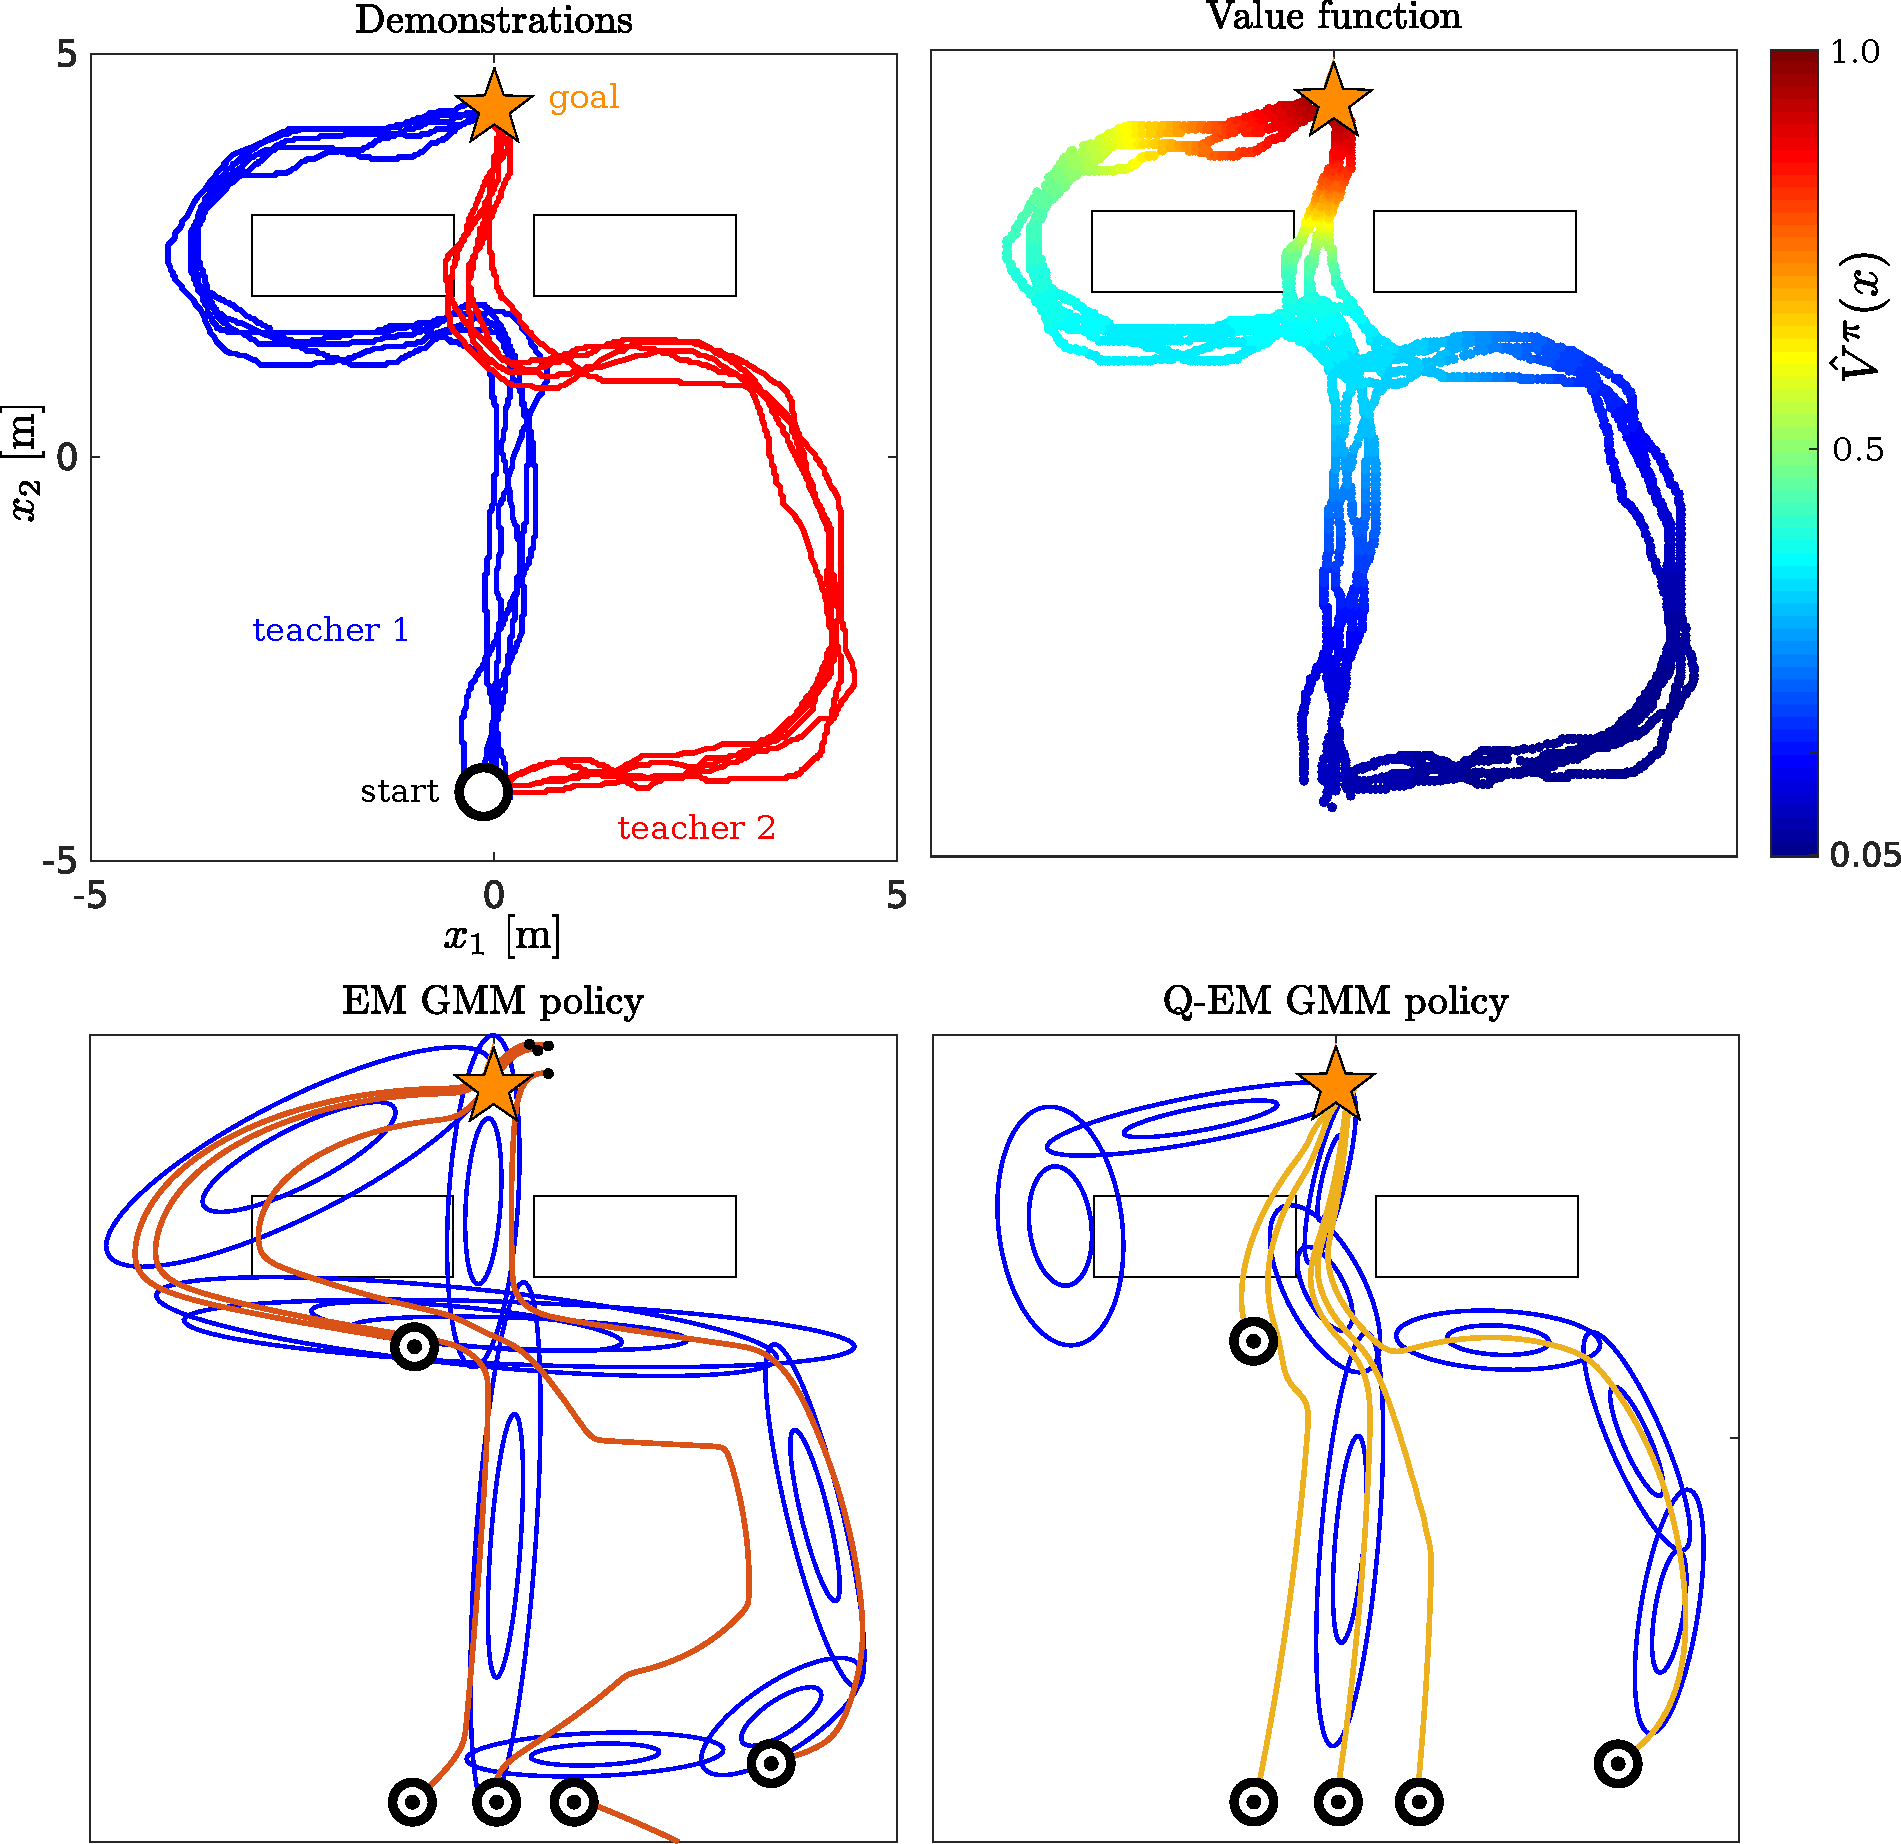
\includegraphics[width=\linewidth]{./Figure/fpe_example.pdf}
 \caption{Fitted policy evaluation \& improvement example. 
  \textit{Top-left:} The goal of the task is to reach the goal state. The first teacher (blue) demonstrates 
  five trajectories which contours the obstacle in front of the goal. The second teacher (red) demonstrates 
  5 trajectories which initially deviate from the goal before passing between the two obstacles. 
  \textit{Bottom-left:} The EM algorithm is used to fit a GMM to the teachers' original data. 
  The marginal $\pi_{\Param}(\X)$ is plotted in blue and trajectories generated by the 
  policy $\mathbb{E}\{\pi_{\Param}(\U|\X)\}$ in orange. \textit{Top-right} \textit{Policy Evaluation:}.  
  Value function after fitted policy evaluation terminated, the reward function 
  is binary, $r=1$ at the goal and zero otherwise, and a discount factor $\gamma = 0.99$ is used.
  \textit{Bottom-right} \textit{Policy Improvement:} the GMM is learned with the Q-EM algorithm in which 
  each data point's weight proportional to the advantage function.
 }
  \label{fig:fpe_example}
\end{figure}

\paragraph{Belief state fitted policy evaluation}

FPI is applied to the data from demonstrations done on socket A. In Figure \ref{fig:ch4:Figure1}  we illustrate the value function 
of the most likely state. As expected, the value function is high closest to the socket and around the axis $z=0$ and $y=0$. 
When policy improvement via Q-EM is applied the Gaussian functions of the GMM will favour these locations. 

\begin{figure*}
 \centering
 
\includegraphics[width=\linewidth]{./Figure/value_function_belief.pdf}
 \caption{\textit{Left}: LWR value function approximate $\hat{V}^{\pi}(\hat{x})$ for the most likely state $\hat{x}$. 
 The red plane is to help visualise where the value function is above and below the axis $z=0$. Only states with values above
 $0.25$ are plotted.  The red arrow indicates the heading of the human teacher when performing the search task. The discount 
 factor was $\gamma=0.99$ and the variance of the kernel variance of 1 [cm], which was set experimentally.
 \textit{Middle-right}: Best and worst trajectories. The red demonstrated trajectories are the best in terms of the amount of value function 
 gain whilst the blue are the worst. The red arrow indicates the teacher's heading. The blue trajectories tend 
 towards the sides of the wall as the initial starting position is on the boarders of the wall. The red trajectories are centred along the y-axis of socket and tend to move in a straight line towards 
 the wall whilst aligning themselves with the axis $z=0$.
}
 \label{fig:ch4:Figure1}
\end{figure*}

In Figure \ref{fig:ch4:Figure1} (\textit{Middle}-right) we illustrate the best and worst trajectories in terms of the accumulated value function.
We can see that the five best trajectories (red) tend to be aligned with the socket (star position in front of socket), 
whilst the worst trajectories are towards the edges of the wall and tend to follow spiralling movements. 

We learned two policies, one solely from the original human demonstrations which we call GMM and the second which 
is the result of \textbf{one iteration} of fitted policy iteration which we call Q-EM. 

\section{Control architecture}\label{ch4:control_architecture}

%As detailed in Section \ref{sec:fpe}, a Gaussian Mixture Model was learned for both linear and angular velocity,
%although only the linear control policy is active until the plug is within 
%the socket's hole, as the orientation is constant.
The direction to search is given by the conditional, Equation \ref{eq:gmm_conditional},

\begin{equation}\label{eq:gmm_conditional}
 \pi_{\Param}(\dot{x}|b) = \sum_{k=1}^{K} w^{[k]}_{\xb} \; g(\dot{x};\MuK_{\xb},\SigK_{\xb}) 
 \end{equation}

which is a distribution over the possible normalised velocities. The function $g(\cdot)$ is a multivariate
Gaussian function parameterised by mean $\MuK_{\xb} \in \mathbb{R}^{(3\times1)}$ and Covariance $\SigK_{\xb} \in \mathbb{R}^{(3\times3)}$. The subscript $\xb$ indicates that the parameters 
are the result of the conditional. The reader is referred to \cite{gesture_calinon_2010}, \cite{gmr_2004} for 
a detailed derivation of the conditional of a GMM. The learned model 
is multi-modal, as different search velocities are possible 
in the same belief state. Figure \ref{fig:policy_vf} illustrates the multi-modal 
vector fields of the conditional, Equation \ref{eq:gmm_conditional}.
In autonomous dynamical systems control, the velocity is obtained from 
the expectation of the conditional, Equation \ref{eq:gmm_conditional}. However, the expectation which is a weighted 
linear combination of the modes, could result in unobserved behaviour or no movement if the velocities cancel out. 
As a result we use a modified version of the expectation operator which favours the current
direction, Equation \ref{eq:alpha_eq} - \ref{eq:alpha_expectation}.

\begin{align}
 \alpha(\dot{x}) &= w^{[k]}_{\xb} \cdot \exp(-\cos^{-1}(<\dot{x},\MuK_{\xb}>)) \label{eq:alpha_eq}\\
 \dot{x} &= \mathbb{E}_{\alpha}\{\pi_{\Param}(\dot{x}|b)\} = \sum_{k=1}^K \alpha_k(\dot{x}) \cdot \MuK_{\xb} \label{eq:alpha_expectation}
\end{align}

When the applied velocity mode is no longer present another direction is sampled. For example, when the robot enters in contact 
with a feature, greatly reducing the uncertainty, the current mode changes and a new search direction is computed. 
Figure \ref{fig:policy_vf} illustrates the policy vector field for GMM and Q-EM, both learned from teachers demonstrations.

\begin{figure}
   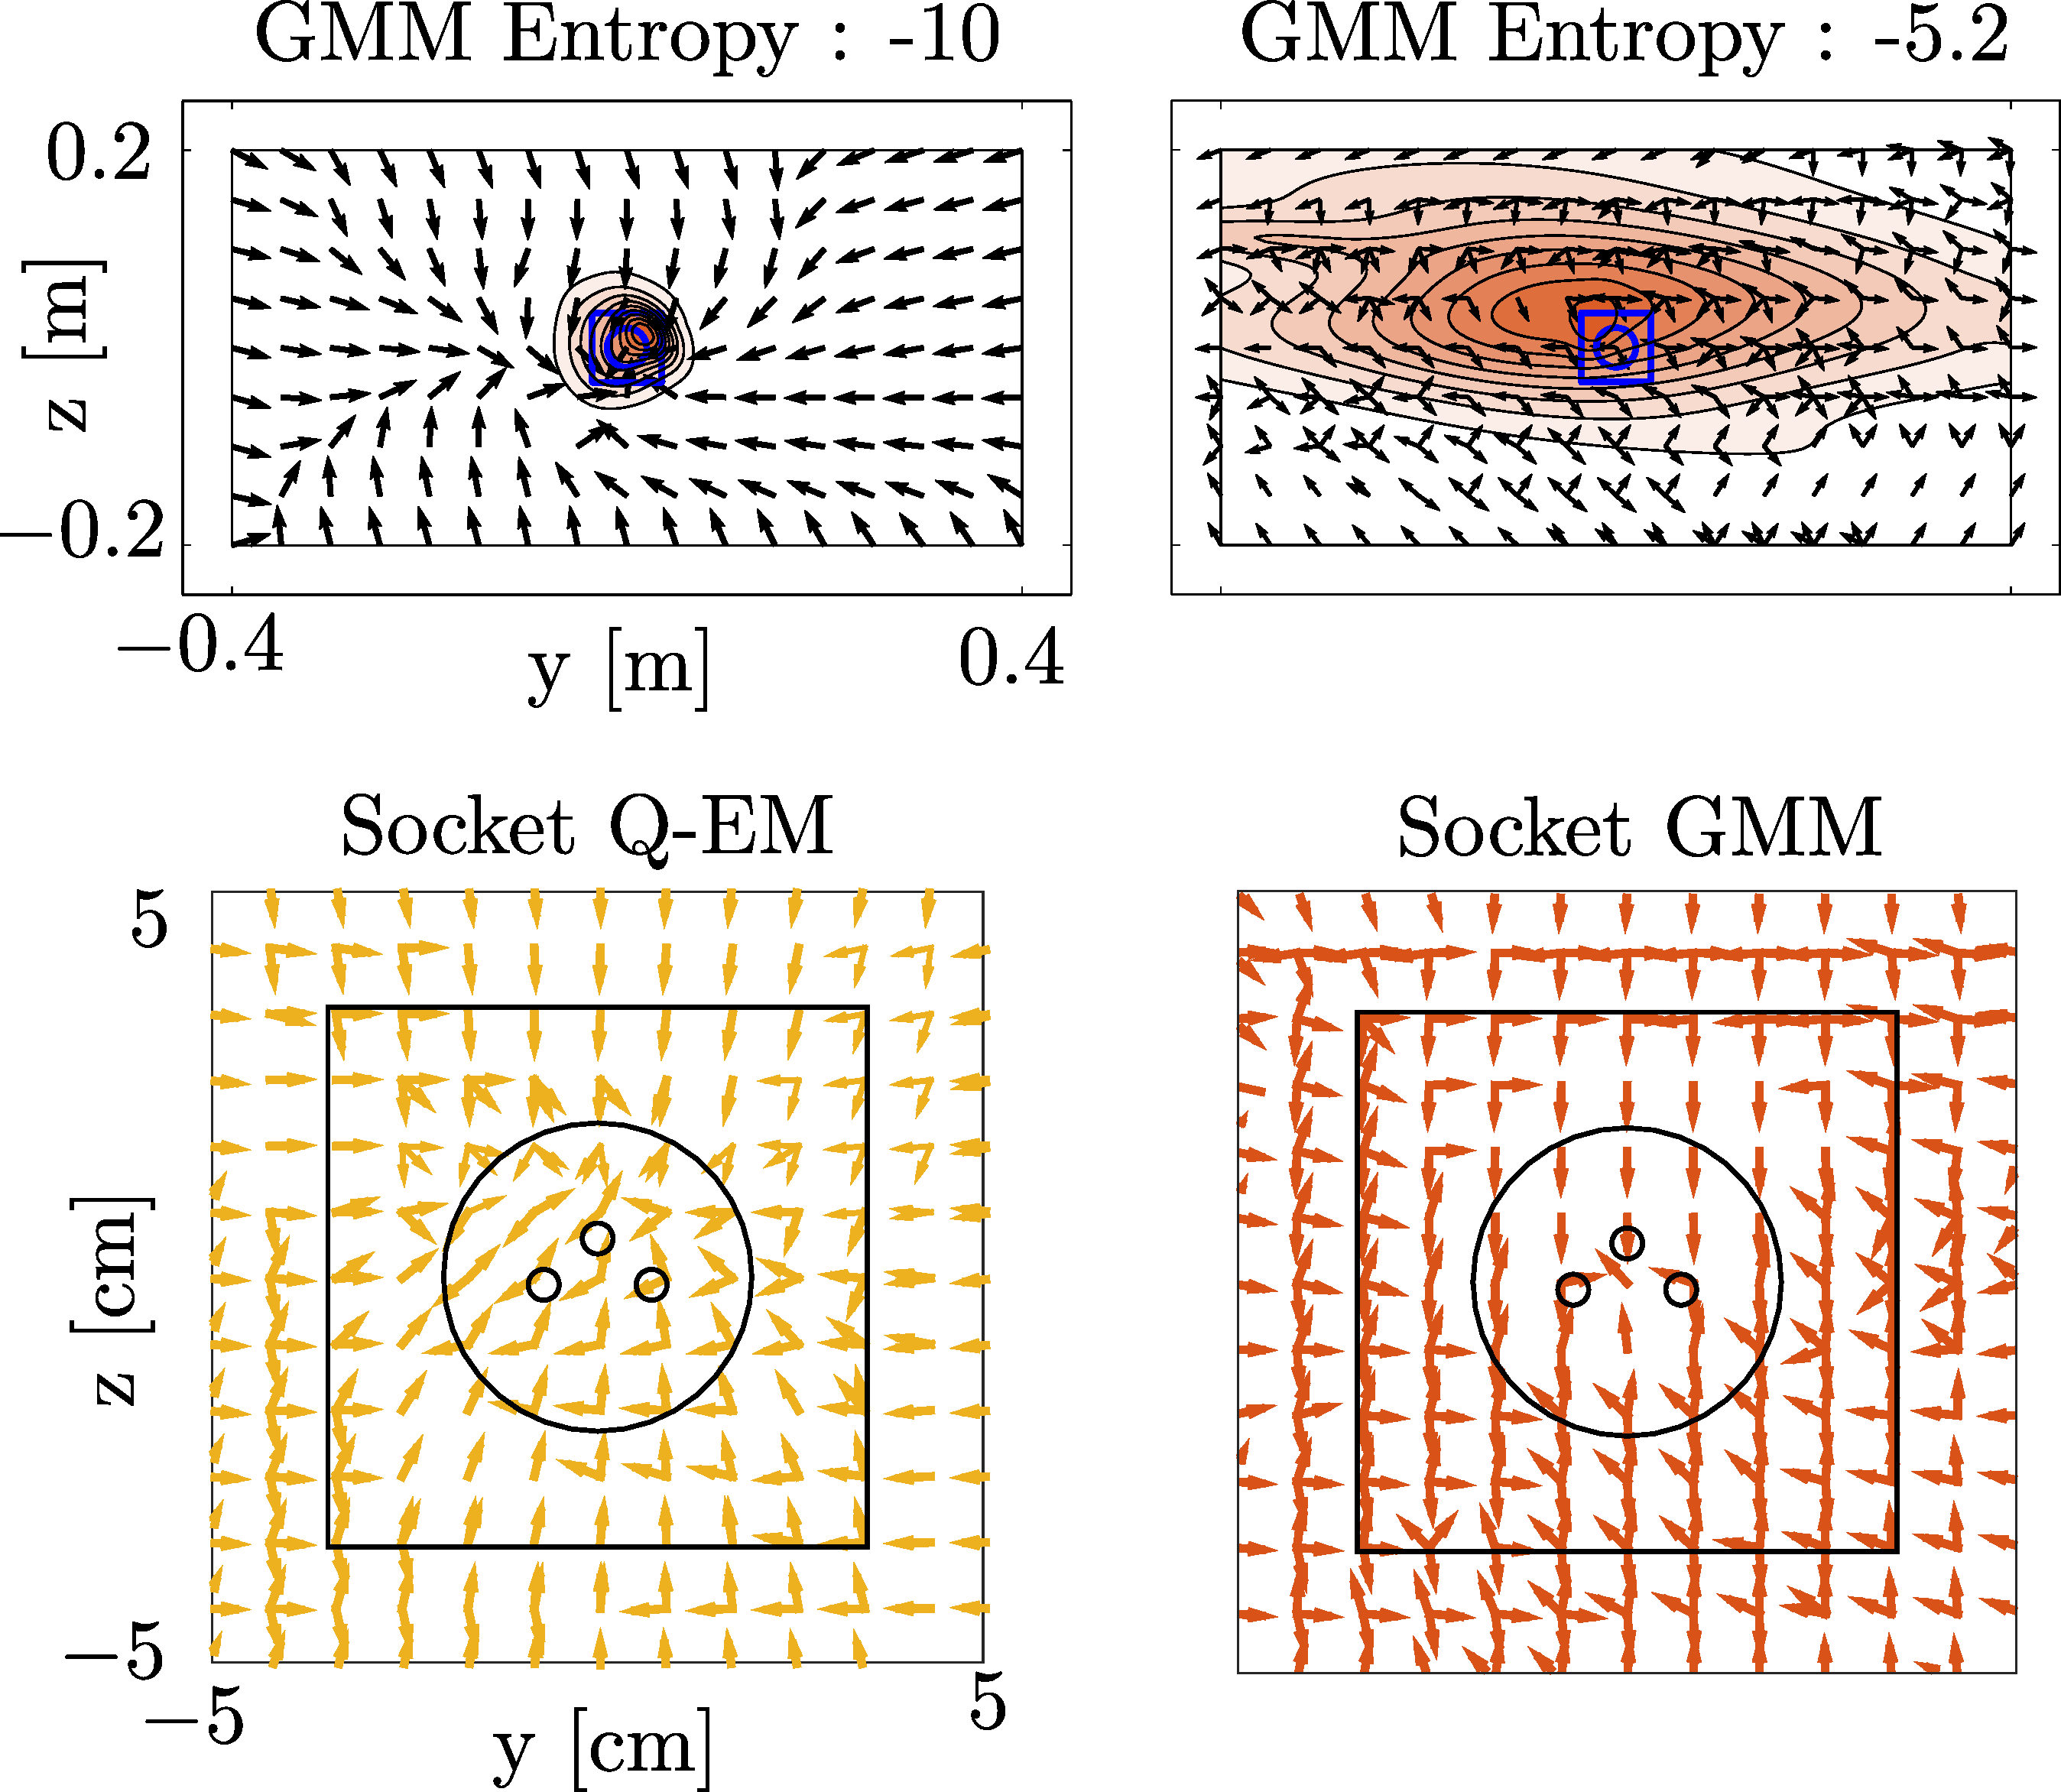
\includegraphics[width=0.45\textwidth]{./Figures/Fig/policy_vf.pdf}
  \caption{Q-EM and GMM policy vector fields. \textit{Top}: The GMM policy is conditioned on an entropy of $-10$ and $-5.2$. For the lowest entropy level,
  most of the probability mass is close to the socket area since this level corresponds to very little uncertainty; we are already localised. We can see 
  that the policy converges to the socket area regardless of the location of the believed state. For an entropy of $-5.2$ we can see that 
  the likelihood of the policy is present across wall. The vector field directs the end-effector to go towards the left or right edge of the wall. 
  \textit{Bottom}: The entropy is marginalised out, the yellow vector field is of the Q-EM and orange of the GMM. The Q-EM vector field tends 
  to be closer to a sink and there is less variation.}
  \label{fig:policy_vf}
\end{figure}


\subsection{Robot Implementation}

The GMM policy $\dot{\underbar{x}} = \mathbb{E}_{\alpha}\{\pi_{\Param}(\dot{x}|b)\}$ outputs a linear velocity which 
is normalised, $\dot{\underbar{x}} \in \mathbb{R}^{(3 \times 1)}$. The amplitude of the velocity is computed separately and 
modulated according to sensed forces on the end-effector.
This search task is haptic and the end-effector of the robot is always in contact with the environment. To make the robot
compliant with the environment we use an impedance controller in combination with a hybrid position-force controller. A hybrid controller
targets a sensed force $F_x$, in the $x$-axis, of 3N. The $y$ and $z$ velocity components of the direction vector are given by 
Equation \ref{eq:alpha_expectation}. This is insufficient for the robot to reliably surmount the edges of the socket,
hence the vector field of the GMM is modulated in $y$ and $z$-axis, Equation \ref{eq:modulation}.

\begin{equation}
  \dot{\underbar{x}} = R_y(c(F_z) \cdot \pi/2) \cdot R_z(c(F_y) \cdot \pi/2) \cdot \dot{\underbar{x}} \label{eq:modulation}
\end{equation}

where $R_y$ and $R_z$ are $(3 \times 3)$ rotation matrices around the $y$ and $z$-axis, and $c(F) \in [-1,1]$ is a truncated scaling function of the sensed 
force.  When a force $F_z$ of 5N is sensed, a rotation of $R_y(\pi/2)$ is applied to the original direction resulting in the robot
getting over the edge. The direction velocity is always normalised up to this point. The amplitude of the velocity is a proportional
controller based on the believed distance to the goal. Figure \ref{fig:control_flow} illustrates the complete control flow.

%\begin{align}
%  \nu     &= \max(\min(\beta_1,K_p (x_g - \hat{x}),\beta_2)\label{eq:prop_speed}\\ \nonumber
%  \dot{x} &= \nu \dot{\underbar{x}}
%\end{align}
%where the lower and upper amplitude limits are given by $\beta_1$ and $\beta_2$, $x_g$ is the position of the
%goal, and $K_p$ the proportional gain which was tuned through trials. 

% $\omega_t = \mathrm{angleaxis}(\mathbf{R}^{\mathrm{T}} \mathbf{R}^r)$  $\mathbf{R}^r = I$

%The above procedure can control the general behaviour of the search but is insufficient for a successful implementation on a robotic system 
%such as the 7 Degree of Freedom $q\in\mathbb{R}^7$ KUKA LWR, which we illustrate in Figure \ref{fig:kuka}. 
%The GMM policy $\dot{x} = \mathbb{E}_{\alpha}\{\pi_{\Param_1}(\dot{x}|b)\}$ outputs a linear velocity and the 
%angular velocity is computed from a reference orientation which is constant. When the plug is to be connected to the socket, 
%the angular velocity is the output of samples drawn from the conditional $\omega \sim \pi_{\Param_2}(\omega|\phi)$.
%From both linear and angular velocities a reference position $x^r \in \mathbb{R}^{(3 \times 1)}$ and orientation $R^r \in \mathbb{R}^{(3 \times 3)}$ are computed and used to 
%define a linear and angular error $x_e = x^r - x$, $\psi_e = \mathrm{angleaxis}(R^{\mathrm{T}}R^r)$ by using the  
%the current position $x$ and orientation $R$.
%Given the kinematic chain of the robot, the inverse of the Jacobian $J(q) \in \mathbb{R}^{6\times 7}$ is used in an impedance control to transform the 
%Cartesian error $c_e = [x_e,\psi_e]^{\mathrm{T}} \in \mathbb{R}^{6 \times 1}$ to torque commands $\tau_t \in \mathbb{R}^7$, Equation \ref{eq:torque_control},
%\begin{equation}\label{eq:torque_control}
% \tau_t = J^{\mathrm{T}}(q_t)\left(-K c_e - D \dot{c}_e \right) + g(q_t)
%\end{equation}
%where $K,D \in \mathbb{R}^{6\times6}$ are diagonal stiffness and damping matrices whose values were set experimentally 
%and $g(q_t)$ compensates for gravity. Given an applied torque there is a resulting joint velocity $\dot{q}_t$ from which we can compute the measured Cartesian end-effector velocity used in the motion model of the PMF.

\begin{figure}
  \centering
  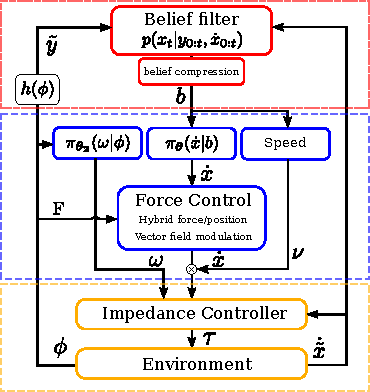
\includegraphics[width=0.45\textwidth]{./Figures/control_flow_final.pdf}
  \caption{Control architecture. The PMF (belief) receives a measured velocity, $\dot{\tilde{x}}$, and 
  a sensor measurement $\tilde{y}$ and is updated via Bayes rule. The belief is compressed and used by 
  both the GMM policy and the proportional speed controller.}
  \label{fig:control_flow}
\end{figure}


\section{Results}\label{sec:results}

We evaluate the following three aspects:
\begin{enumerate}
 \item \textbf{Distance taken to accomplish the goal} (connect plug to socket). We compare the Q-EM policy with 
 a GMM policy learned through standard EM and a myopic Greedy policy. This highlights the difference between complicated and simplistic  
  search algorithms and gives an appreciation of the problem's difficulty.
 \item \textbf{Importance of data} provided by human teachers. We evaluate whether it is possible to learn 
 an improved GMM policy from Greedy demonstrations. This policy which we call Q-Greedy is used to test whether 
 indeed human demonstrations are necessary. We evaluate whether it is possible to obtain a good policy from the two worst teachers' demonstrations as not all teachers 
 are necessarily proficient at the task in question. 
  \item \textbf{Generalisation}. We learn a policy to insert a plug into socket A which is located at the center of a wooden 
 wall. We test the generalisation of the policy in finding a new socket location and whether the policy can generalise to sockets 
 B and C, which were not used during the training phase.
\end{enumerate}

We evaluate aspects 1) and 2) purely in simulation as finding the socket requires much less precision than establishing a 
connection and the physics of the interaction is simple. Aspect 3), the generalisation, is evaluated both in simulation,
up to the point of localising the socket's edge, and on the KUKA LWR robotic platform
for the connection phase of the task. The main reason for employing the robot is that the connection phase dynamics is 
complex and a simulation would be unrealistic. For the robot evaluation we consider 
the search starting already within the vicinity of the socket.

\subsection{Distance taken to reach the socket's edge}

We consider two search experiments which we refer to as \textbf{Experiment 1} and \textbf{2}, in order to evaluate the performance 
in terms of the distance travelled to reach the socket for the three search policies: GMM, Q-EM and Greedy. In these two 
experiments the task is considered accomplished when a search policy finds the socket's edge. 

\textbf{Experiment 1}, three starting locations are chosen: \textit{Center}, \textit{Left} and \textit{Right}. 
See Figure \ref{fig:experiment12} \textit{(Experiment 1 Top-left)}, for an illustration of the initial condition. 
This setup tests the effect of the starting positions. A total of 25 searches are carried out for each of the search policies.
The trajectory results show a clear difference between the trajectories generated by the GMM and Q-EM policies (\textit{Experiment 1 Bottom-left}). 
The orange GMM policy trajectories go straight towards the wall, whilst the yellow Q-EM policy trajectories drop in height 
making them closer to the socket. 
\textit{Experiment 1 Bottom-right}, we illustrate the distribution of the first contact with the wall for the \textit{Center} initial 
conditions. The distribution of the first contact of the Greedy method is uniform across the entire $y$-axis of the wall. 
It does not take into account the variance of the uncertainty. In contrast, the GMM policy remains centred 
with respect to the starting position and the Q-EM is even closer to the socket and there is much less variance in 
the location of the first contact.

\textit{Experiment 1 Top-right}, we illustrate the quantitative results of the distance taken to reach the socket for 
all three experiments. For the \textit{Center} initial condition, the Q-EM policy travels far less than the other search policies. 
Considering that the initial position of the search is 0.45 [m] away from the wall, the Q-EM policy finds the socket very 
quickly once contact has been established with the wall. For the \textit{Right} and \textit{Left} starting conditions both 
the GMM and Q-EM policies travel less distance to reach the socket, with a smaller variance when compared with the Greedy search policy.

\textbf{Experiment 2}, Figure \ref{fig:experiment12} (\textit{Experiment 2}), the initial true starting positions 
of the end-effector are taken from a regular grid, within the red cube (see \textit{Experiment 1}), covering the whole start region, also used as the initial distribution for 
the human demonstrations. A total of a 150 searches are carried out for each of the three policies. 
This experiment compares the search policies with the human teachers' demonstrations. 
The Human and GMM show similar distributions of searched locations. They cover the upper region of the wall and top corners, to some extent. These distributions 
are not identical for two reasons. The first is that the learning of the GMM is a local optimisation 
which is dependent on initialisation and number of parameters. The second reason is that the synthesis of trajectories 
from the GMM is a stochastic process. 

For the  Q-EM policy, the distribution of the searched locations is centred around the origin of the $z$-axis.
The uncertainty is predominantly located in the $x$ and $y$-axis. The Q-EM policy takes this uncertainty 
into consideration by restraining the search to the $y$-axis regardless of the starting position. The uncertainty 
is reduced when it is in the vicinity of the socket. The Greedy's policy search distribution is multi-modal and 
centred around the $z$-axis where the modes are above and below the socket. This shows that the Greedy policy 
acts according to the most likely state which changes from left to right of the socket, because of motion noise, 
resulting in left-right movements and little displacement. As a result the Greedy policy spends more time at these modes.

\textit{Experiment 2 Right}, it is clear that all three search policies travel less to find the socket's edge compared 
with the teachers' demonstrations. All search policies are better than the human teachers with the exception of group BA, 
which is performing the task with socket A. The Q-EM policy remains the best. 

\begin{figure*}
    \centering
    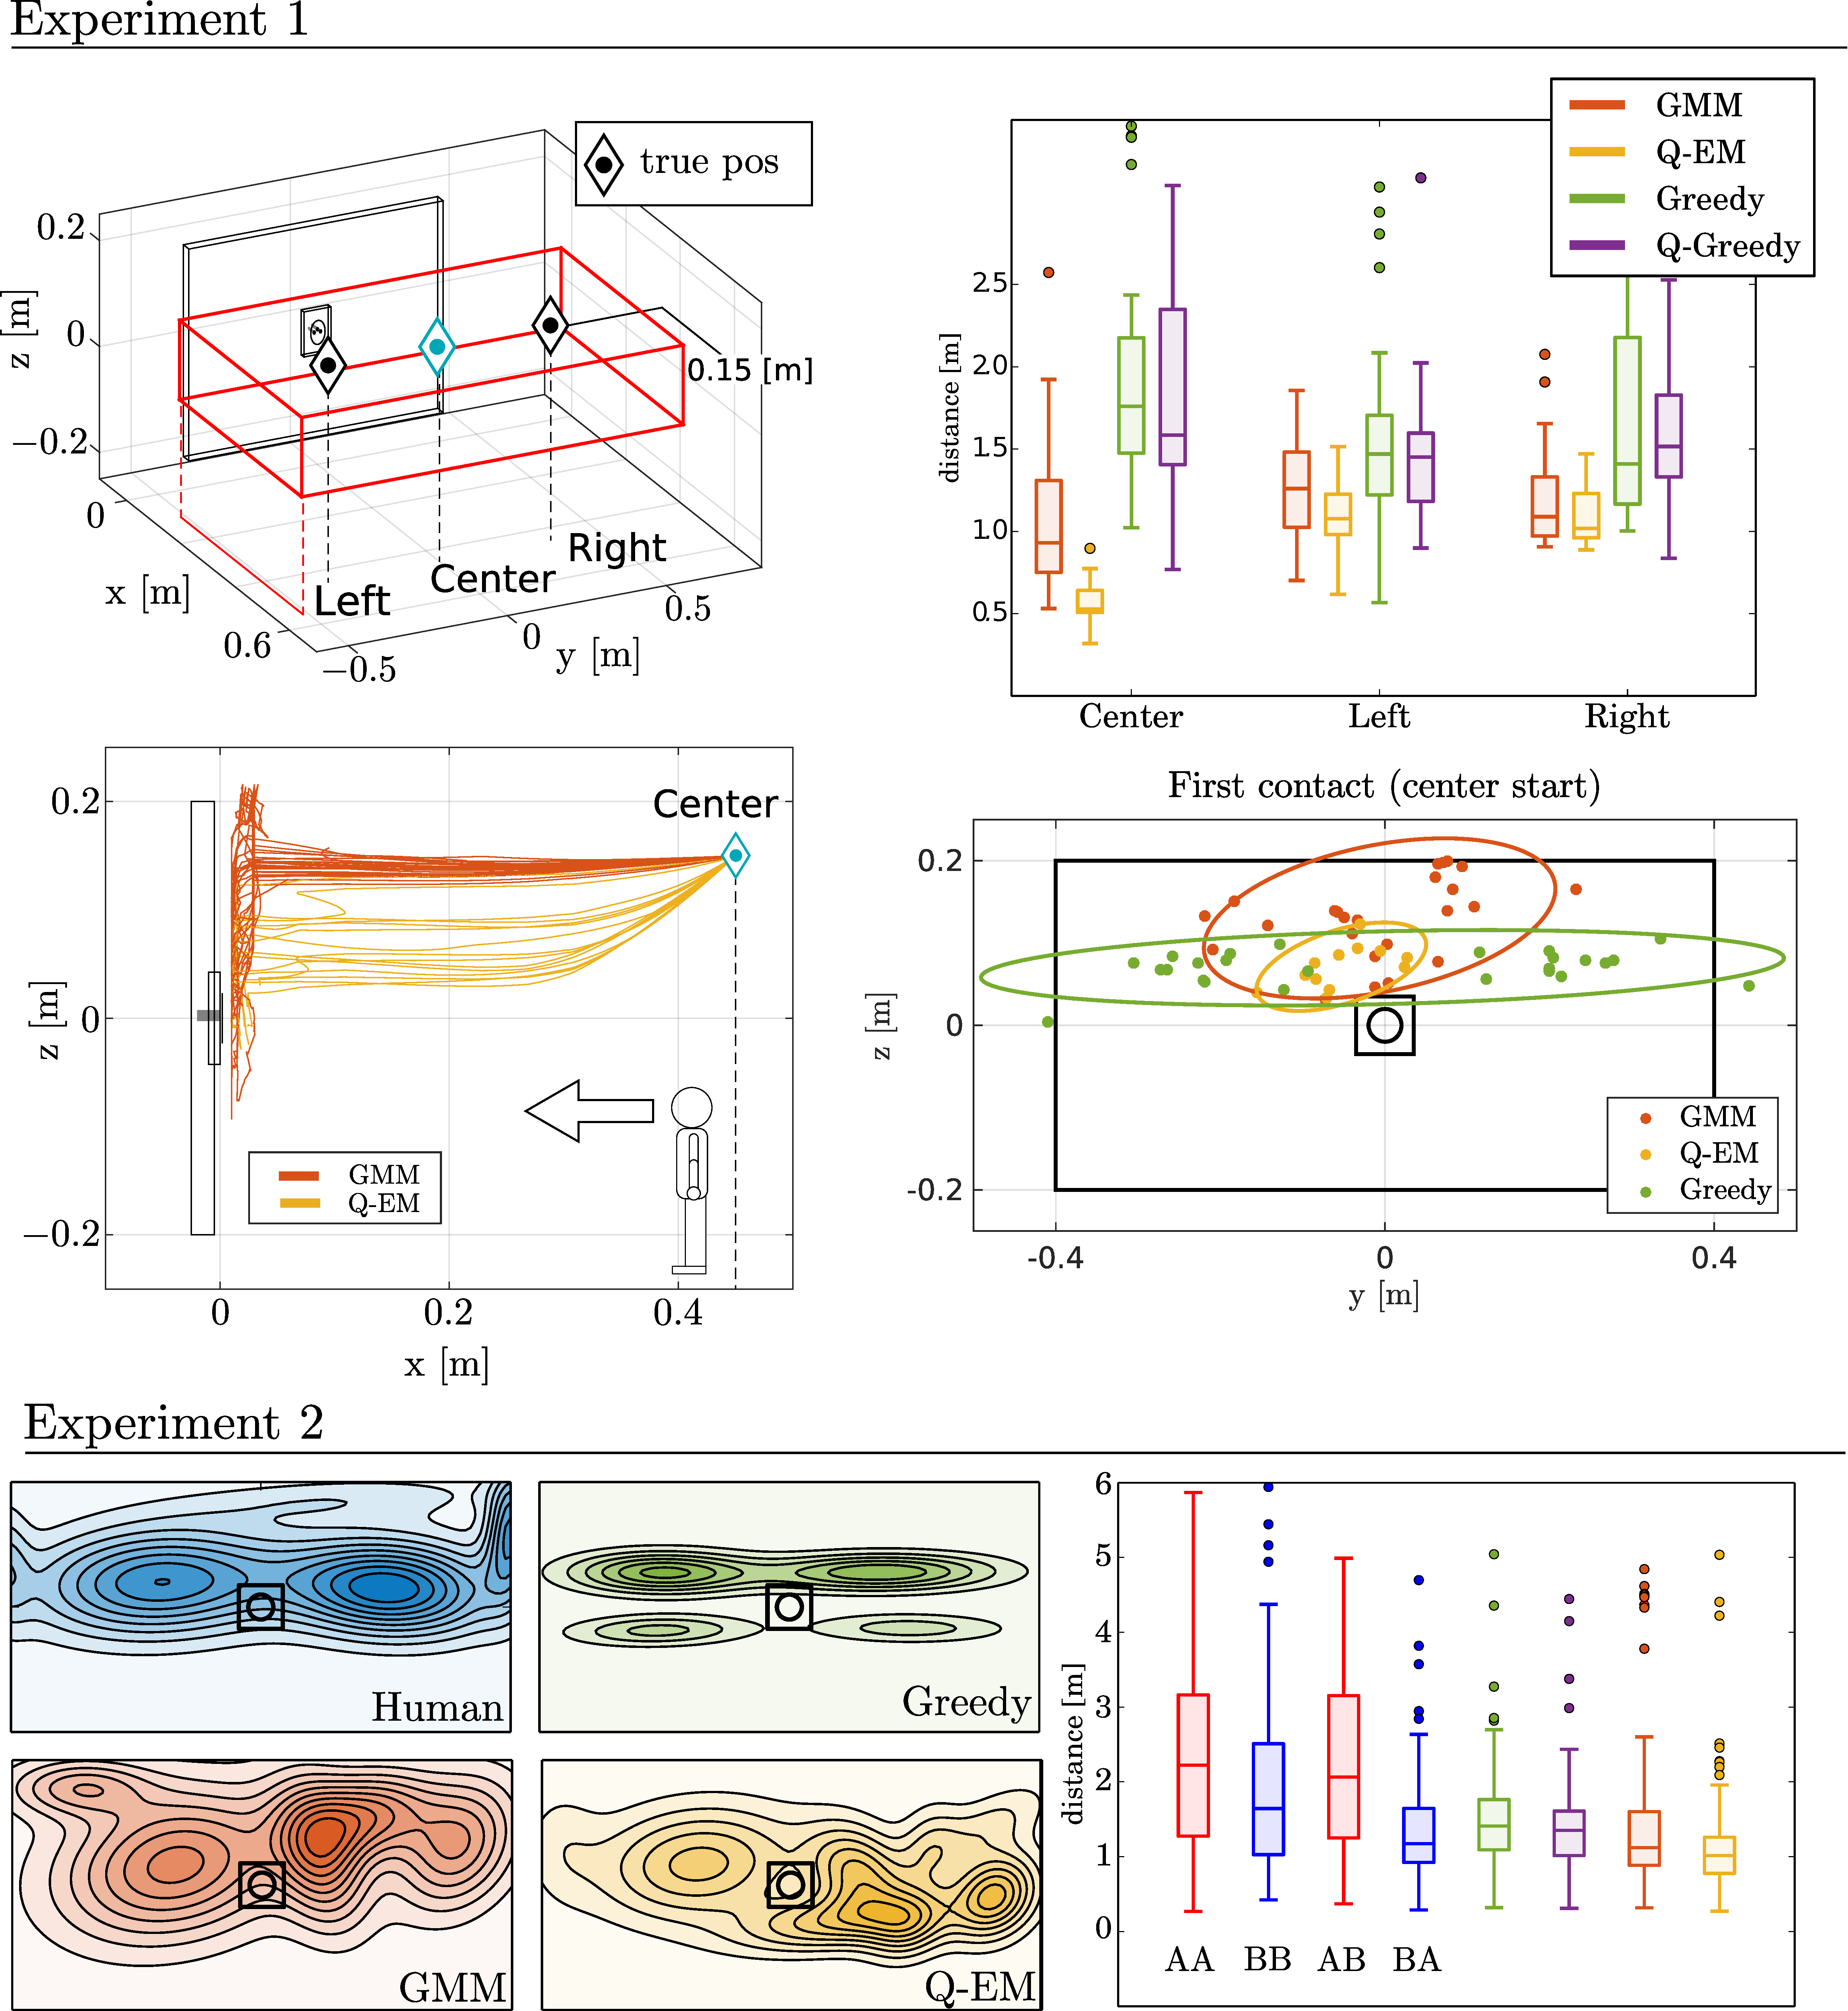
\includegraphics[width=\linewidth]{./Figure/experiment1.pdf}
    \caption{Two simulated search experiments. \textbf{Experiment 1:} \textit{Top-left}: 
     Three start positions are considered: \textit{Left}, \textit{Center} and \textit{Right} in which the triangles depict true position of the end-effector. 
     The red cube illustrates the extent of the uncertainty. \textit{Bottom-left}: Trajectories of both the GMM (orange) and Q-EM (yellow) policies. 
     For each start condition a total of 25 searches were performed for each search policy.
     \textit{Bottom-right:} Distribution of first contact point giving the center initial starting condition. \textit{Top-right}: Distribution of distance 
     travelled until the socket's edge was localised. The Q-EM policy is always the best.
     \textbf{Experiment 2}: \textit{Left}: Distribution of the visited regions during the search for the socket's edge. The Q-EM policy's distribution 
     is more centred along the axis $z=0$. \textit{Right:} Time taken to find the socket, the search algorithms are better than the humans with the exception 
     of group BA.} 
    \label{fig:experiment12}
\end{figure*}

We have shown that under three different experimental settings the Q-EM algorithm is predominantly the best in terms of distance taken 
to localise the socket. The GMM policy learned solely from the data provided by the human teachers also performs well in comparison to  
the human teachers and Greedy policy. We made, however a critical assumption in order to be able to use our statistical policy approach. 
This \textbf{assumption} is that a human teacher is proficient in accomplishing the task. If a teacher is not able to accomplish 
the task in a repetitive and consistent way so that a search patter can be encoded by the GMM, the learned policy will perform poorly.
Next we evaluate the validity of this assumption and the importance of the training data provided by the human teachers.
 
\subsection{Importance of data}

We perform two tests to evaluate the importance of the teachers training data, which we will refer to as \textbf{Experiment 3}.
Firstly we take the worst two teachers in terms of distance taken to find the socket's edge and learn a GMM and Q-EM policy separately from their 
demonstrations. In this way we can evaluate whether it is possible to learn a successful policy given 
a few bad demonstrations (15 training trajectories for each policy). Our second evaluation consists of using a noisy 
explorative Greedy policy as a teacher to gather demonstrations which can then be used to learn a new policy, which we call Q-Greedy. 

Figure \ref{fig:experiment3} (\textit{Top-left}) illustrates 6 trajectories of teacher \# 5. Once localised, the teacher 
would reposition himself in front of the socket and try to achieve an insertion. This behaviour was not expected 
since by losing contact with the wall, the human teacher no longer had sensory feedback necessary 
to maintain an accurate position estimate.

\begin{figure*}
 \centering
    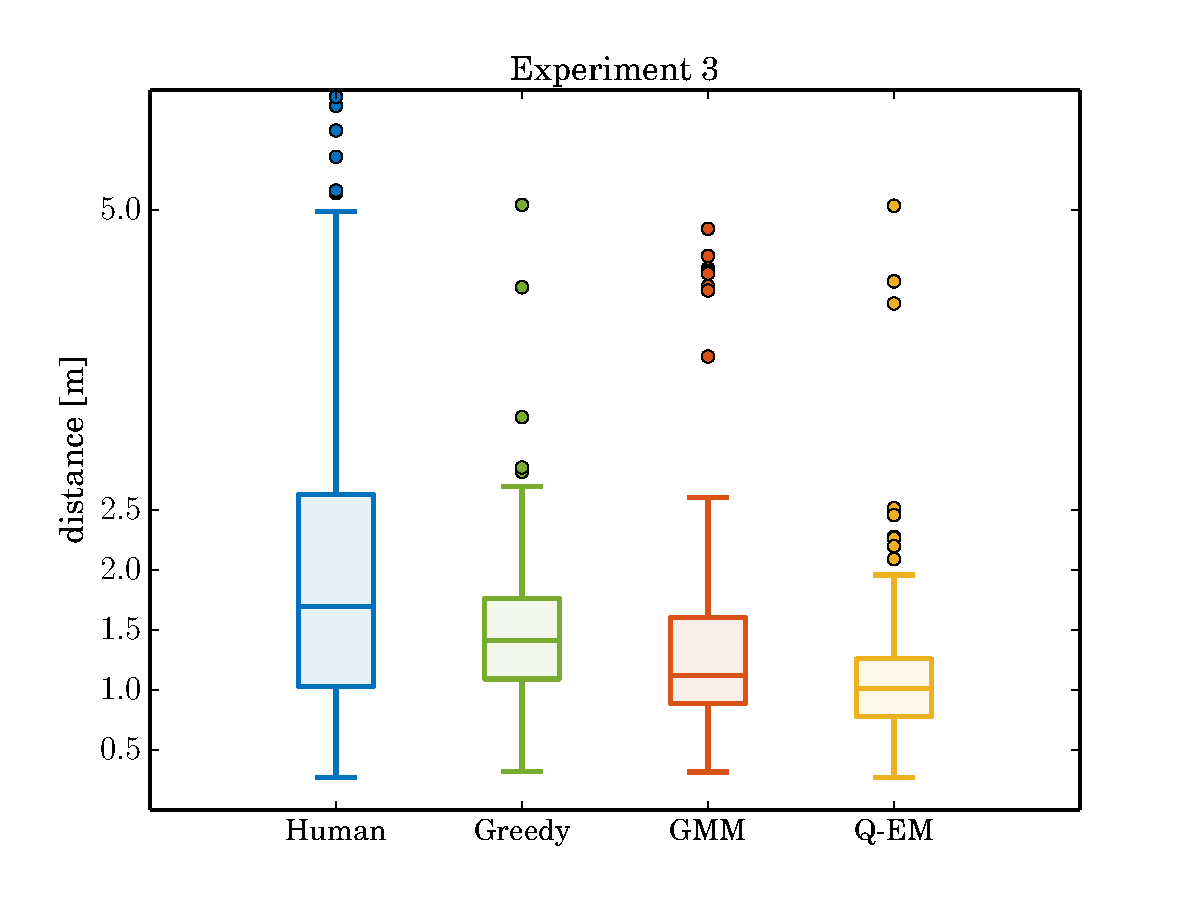
\includegraphics[width=\linewidth]{./Figure/experiment3.pdf}
    \caption{\textbf{Experiment 3} \textit{Top-left}: Demonstrations of teacher \# 5. \textit{Bottom-left} Value function learned from the 15 demonstrations of teacher \#5. The value of the most 
    likely state is plotted. \textit{Middle-column}: Most likely state parameters of the GMM and Q-EM learned from the 
    demonstrations of teacher \#5. \textit{Right-column}: Rollouts of the policies learned from teacher \#5. We can see that trajectories 
    from the GMM policy have not really encoded a specific search patter, whilst the Q-EM policy gives many more consistent trajectories 
    which replicate to some extent the pattern of making a jump (no contact with the wall) from the top right corner to the socket's edge.}
    \label{fig:experiment3}
 \end{figure*}
% \begin{figure}
%    \centering
%    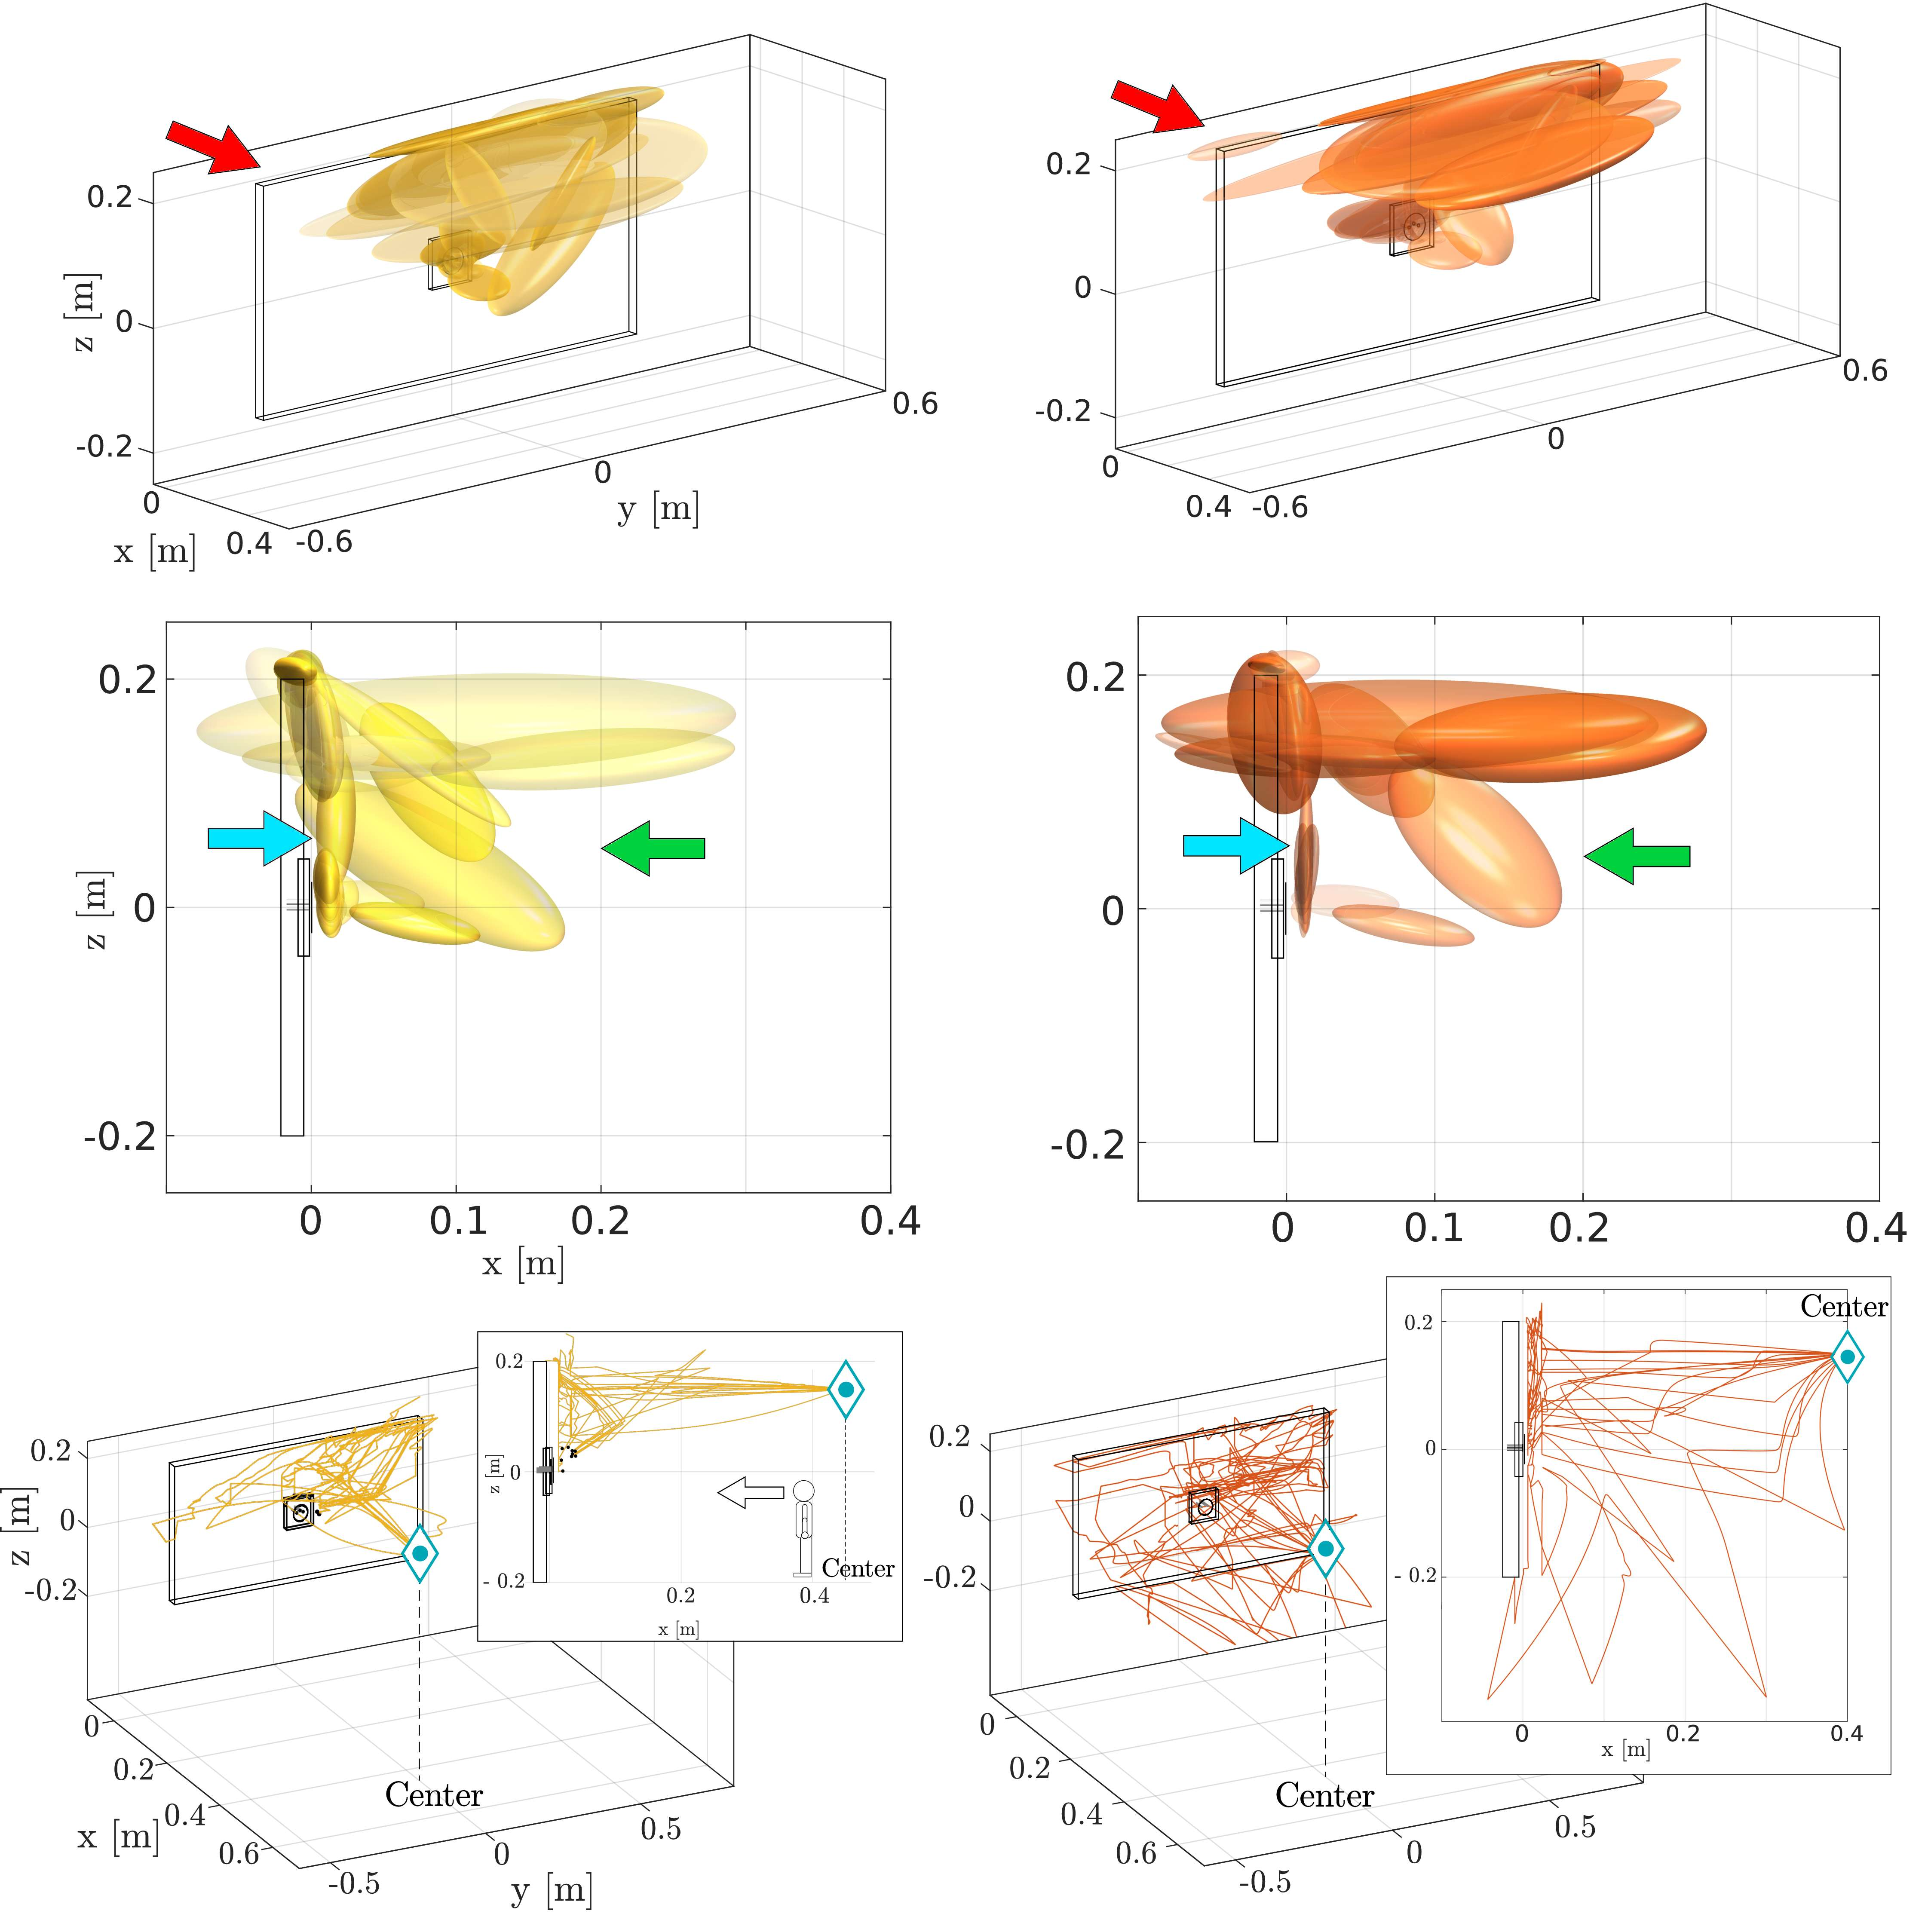
\includegraphics[width=\linewidth]{./Figures/Fig/gmm_v2c.pdf}
%    \caption{Marginalised Gaussian Mixture parameters of the GMM and Q-EM learned from the demonstrations of teacher \#5. 
%    The illustrated transparency of the Gaussian functions is proportional to their weight.
%    \textit{Left column}: The Gaussian functions of the Q-EM have shifted from the left corner to the right. This is a result of the value function 
%    being higher in the top right corner region, see Figure \ref{fig:value_function_subj_5}. \textit{Center column}:  The original data of the teacher 
%    went quite far back which results in a Gaussian function given a direction which moves away from the wall (green arrow), whilst in the case
%    of the Q-EM parameters this effect is reduced and moved closer towards the wall.  We can also see from the two plots of the Q-EM parameters 
%    that they then follow the paths encoded by the value function.    
%    \textit{Right column}: Rollouts of the policies learned from teacher \#5. We can see that trajectories from the GMM policy have not really 
%    encoded a specific search patter, whilst the Q-EM policy gives many more consistent trajectories which replicate to some extent 
%    the pattern of making a jump (no contact with the wall) from the top right corner to the socket's edge.}
%    \label{fig:gmm_exp4}
%\end{figure}
 
Figure \ref{fig:experiment3} (\textit{Bottom-left}) illustrates the value function of the belief state learned from the data of teacher \# 5.
The states with the highest values seem to create a path going from the socket towards the right edge of the wall. 
We proceed as before to learn a GMM policy from the raw data and a Q-EM policy in which the data points are weighted by 
the gradient of the value function. \textit{Experiment 3 Middle-column}, we illustrate the 
resulting Marginalised Gaussian Mixture parameters for both the GMM and Q-EM policies and we plot 25 rollouts of each policy starting at 
the \textit{Center} initial condition used in Experiment 1. We note that the trajectories of the GMM 
policy have much variance in contrast to the Q-EM policy, resulting from an excess of variance in the 15 original demonstrations
given by the teacher. Too much variance is not necessarily good, a random (uniform) policy in terms of generated trajectories
will have the most variance and is as expected extremely inefficient in achieving a goal. Furthermore there is insufficient data to encode a pattern for the GMM model. In contrast, the Q-EM finds a 
pattern by combining multiple parts of the available data and as a result fewer data points are necessary to achieve a good policy. 
This effect is clear in Figure \ref{fig:experiment3_stats}, showing the performance of the GMM and Q-EM algorithms 
under the same initial conditions as in Experiment 1. For all the conditions and for both teachers \#5 and \#7 the Q-EM policy 
always does better than the GMM.

\begin{figure}
 \centering
 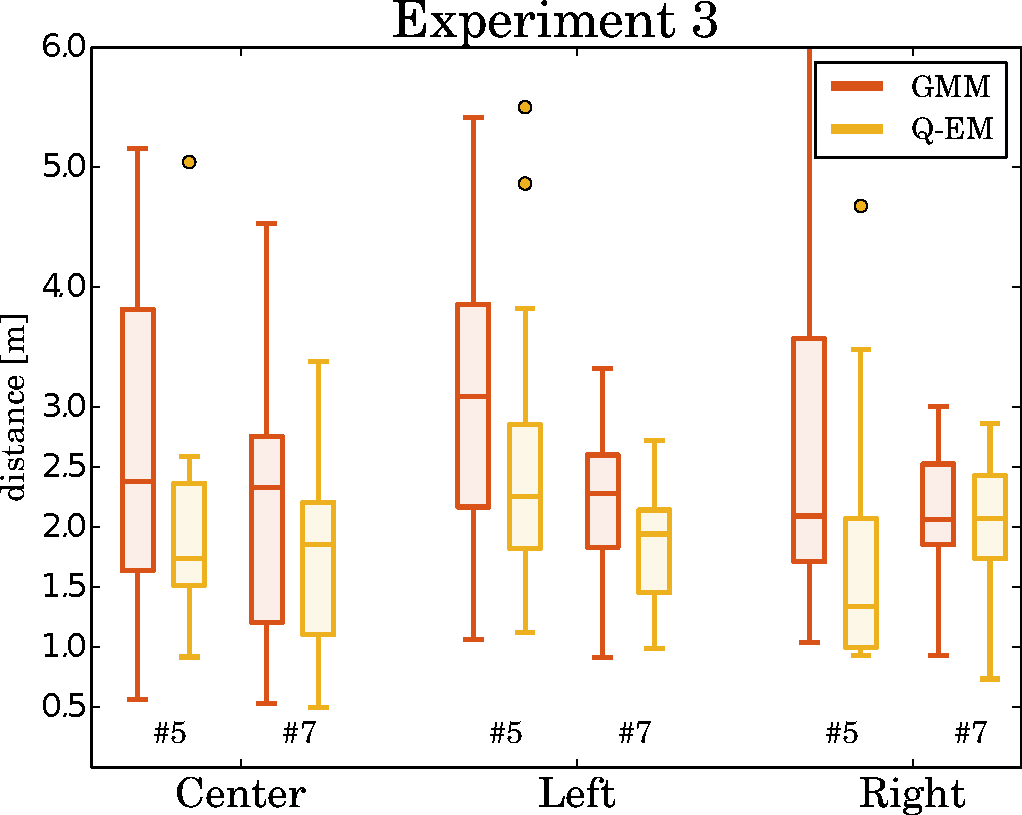
\includegraphics[width=\linewidth]{./Figure/experiment3_stats.pdf}
 \caption{Results of a GMM and Q-EM policy under the same test conditions as Experiment 1. The Q-EM policy nearly always does much better than the GMM policy.}
 \label{fig:experiment3_stats}
\end{figure}

We also tested whether we could use the Greedy policy as a means of gathering demonstrations in order to learn a value function and 
train a Q-Greedy policy. We used the Q-Greedy algorithm in combination with random perturbations applied to the Greedy velocity, to act as 
a simple exploration technique. We performed a maximum of 150 searches, which terminated once the socket was found and used these demonstrations to 
learn a value function and GMM policy which we refer to as Q-Greedy. Figure \ref{fig:experiment12} \textit{Experiment 1-2 (bar plot)}, illustrates the statistical results 
of the Q-Greedy policy for Experiment 1 and 2 (purple bar chart), showing that there is no difference between two policies. 
Our exploration method is probably too simplistic to discover meaningful search patterns and we could probably devise better 
search strategies which would result in a good policy. However we have shown that human behaviour does already have a usable trade-off 
between exploration and exploitation which can be used to learn a new policy through our Fitted Policy Iteration framework.

\subsection{Generalisation}

So far we have trained and evaluated our policy within the same environment.
To test whether our GMM policies can generalise to a new setting we changed the location of the 
socket to the upper right corner of the wall. The GMM was trained in the frame of reference of the socket and
when we translated the socket's location it also translated the policy. 

\begin{figure*}
 \centering
    \subfigure[]{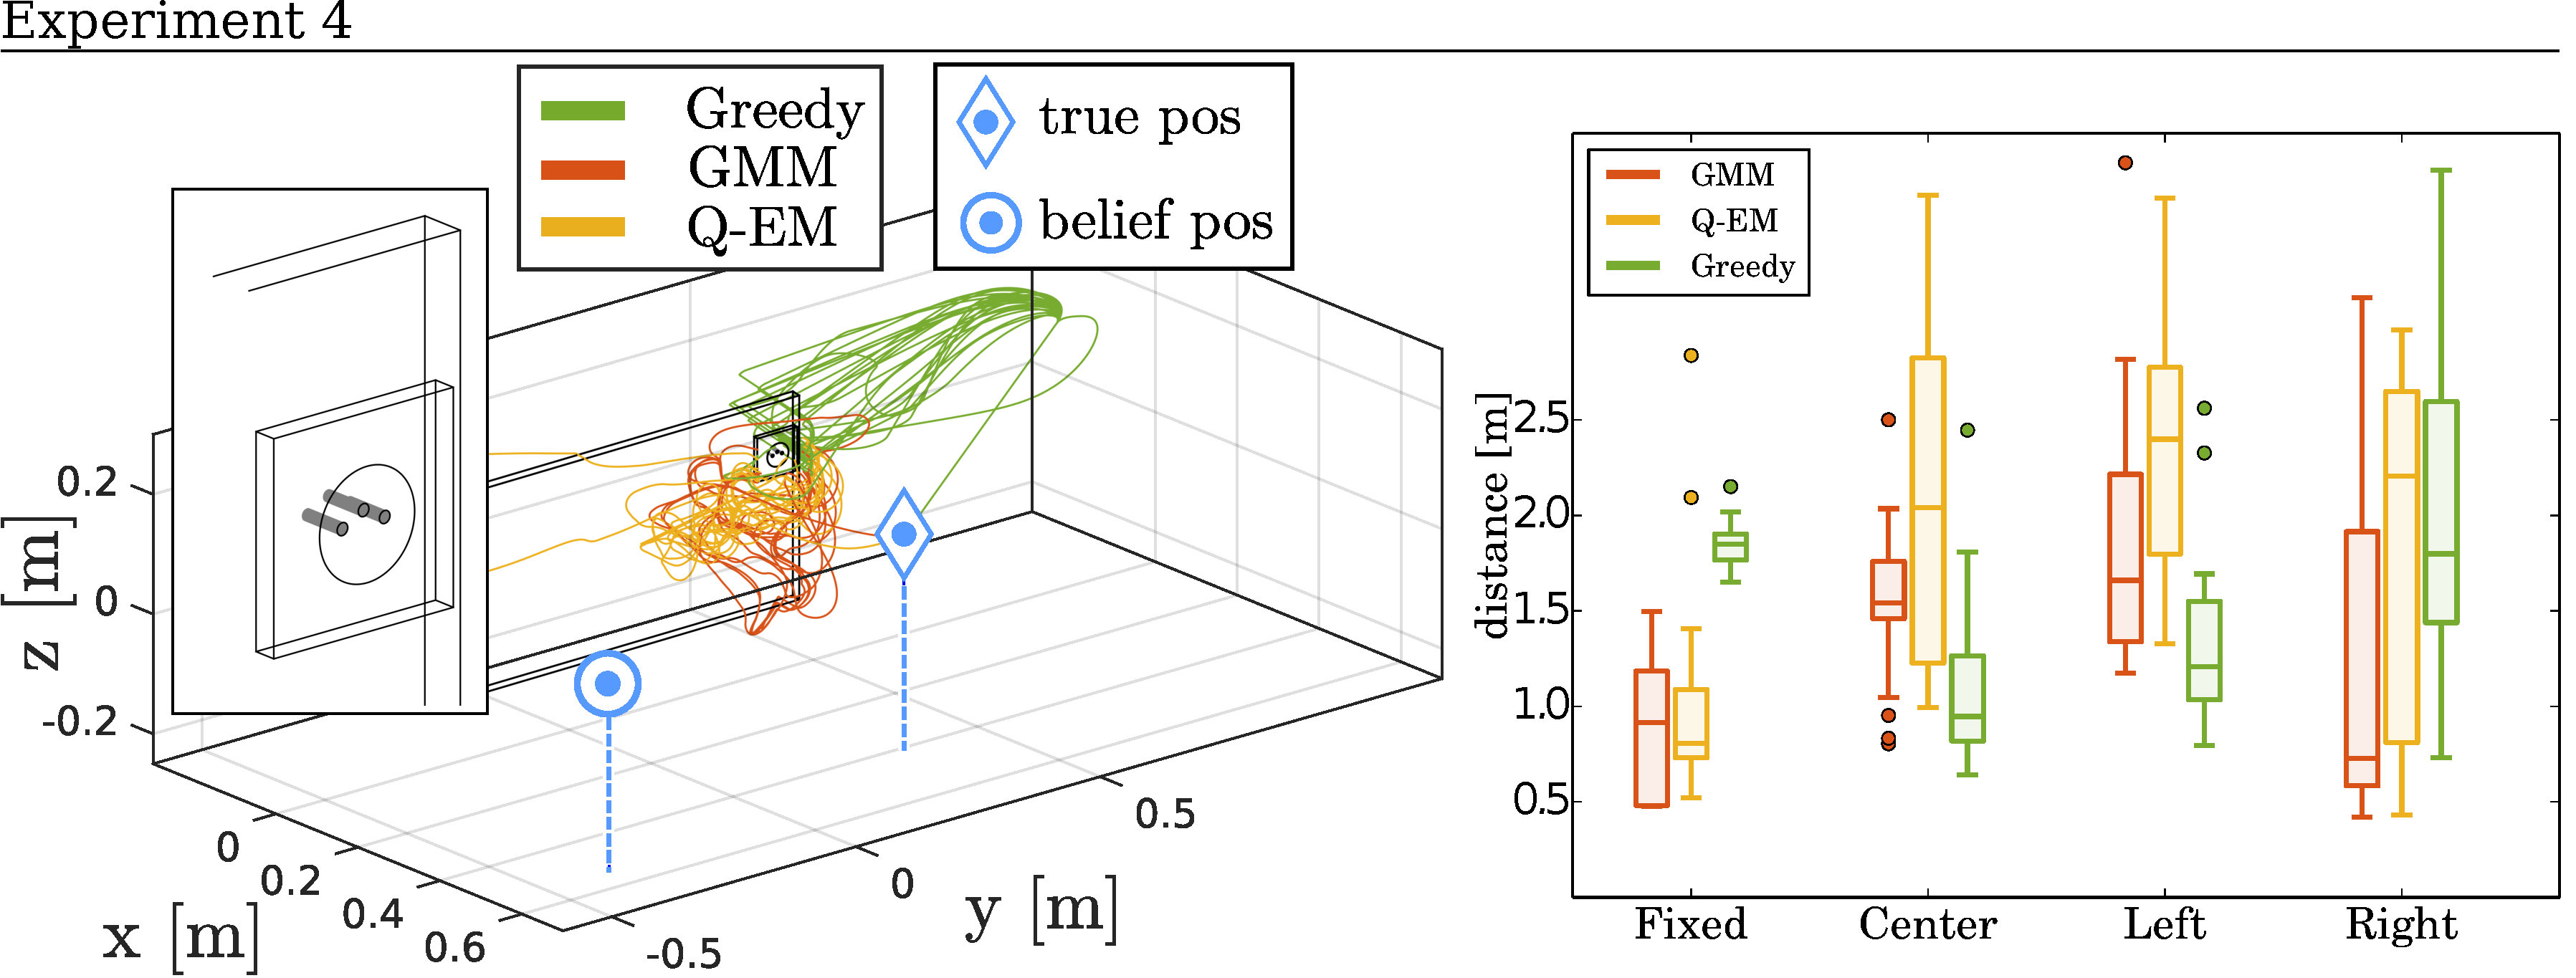
\includegraphics[width=\linewidth]{./Figure/experiment4.pdf}}
    \caption{\textbf{Experiment 4} Evaluation of generalisation. The socket is located in at the top right corner of the wall. We consider a 
    \textit{Fixed} starting location for both the true and believed location of the end-effector. The red square depicts the 
    extent of the initial uncertainty, which is uniform. (b) Distance taken to reach the socket's edge. For the Fixed setup (see (a) for 
    the initial condition), both the Q-EM and GMM significantly outperform the Greedy. The other three conditions are the same as for 
    Experiment 1. }
    \label{fig:experiment4}
\end{figure*}

%\begin{figure}
% \centering
%    \subfigure[]{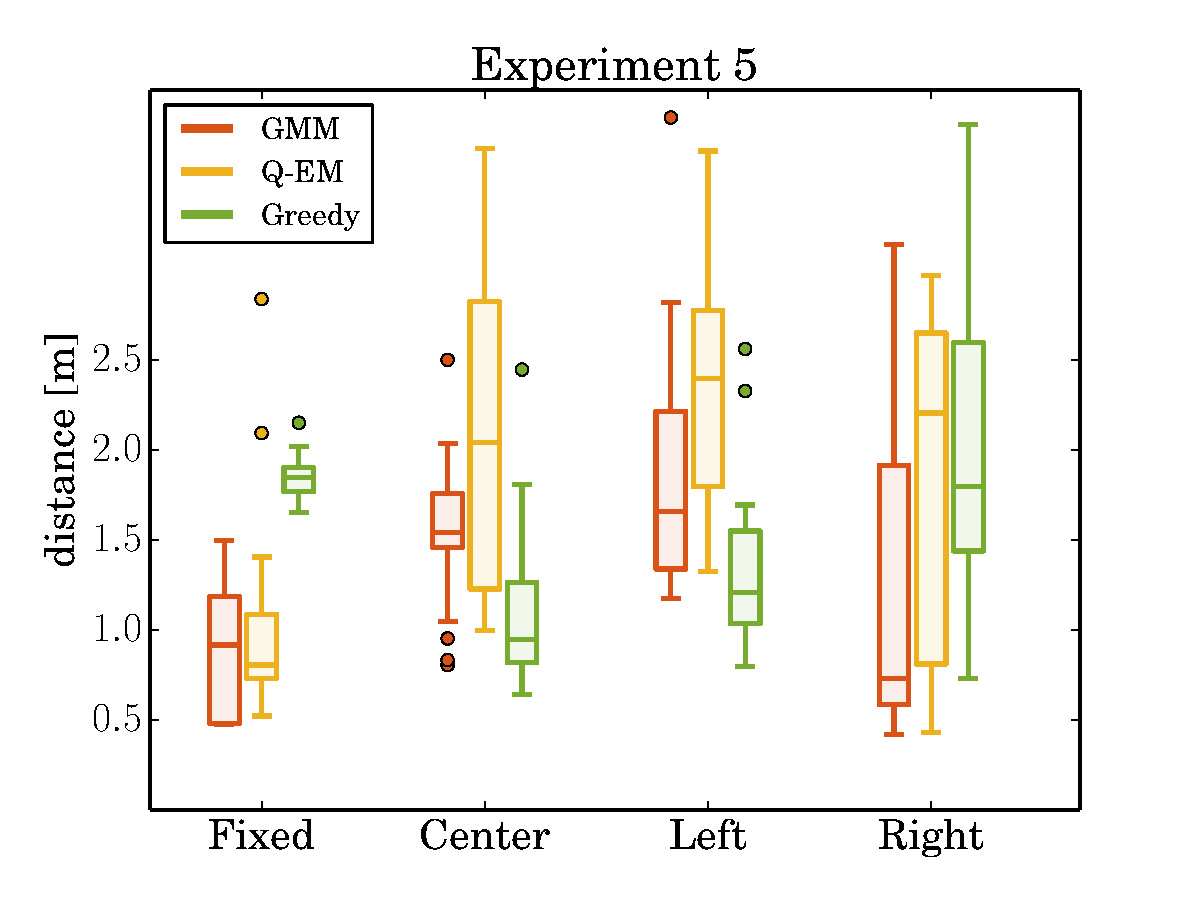
\includegraphics[width=\linewidth]{./Figures/Fig/experiment5.pdf}}
%    \caption{Distance taken to reach the socket's edge. For the Fixed setup (see Figure \ref{fig:experiment4}) for 
%    the initial condition), both the Q-EM and GMM significantly outperform the Greedy. }
%    \label{fig:experiment5_stats}
%\end{figure}

We use the same initial conditions of Experiment 1 with an additional 
new configuration named \textit{Fixed}, in which both the true and believed location are fixed, blue triangle and circle.
Figure \ref{fig:experiment4} \textit{(Left)} illustrates the trajectories of the three search policies for the \textit{Fixed} initial condition. 
The Greedy policy moves in a straight line towards the top
right corner of the table. As the true position is to the right, it takes the Greedy policy longer to find the wall 
in contrast to both the GMM and Q-EM policies. From the statistical results shown in Figure \ref{fig:experiment4} \textit{(Right)} we can see
that for the \textit{Fixed} and \textit{Right} initial condition, which are similar, both GMM and Q-EM are better. However, for 
the \textit{Center} and \textit{Left} initial condition this is no longer the case. 
The Greedy method is better under this condition since the socket is close to informative features (it is located close to the edges of the wall). 
Once the end-effector has entered in contact with the wall the actions of the Greedy policy always result in a decrease of uncertainty, which was not the case when the socket was located in the center of wall. 
Thus in both the \textit{Fixed} and \textit{Right} initial condition the Greedy method does worse because it takes longer
to find the wall.

The GMM based policies are still able to generalise under different socket locations. In general, as the socket's location is moved 
further from the original frame of reference in which it was learned, the higher is the likelihood that the search quality degrades. We 
chose the upper right corner since it is the furthest point from the origin and the GMM and Q-EM policies were still able to find 
the socket. We note that the policy will always be able to find the socket once it has localised itself. This can be seen from the vector field 
of the GMM policy when the uncertainty is low, see Figure \ref{fig:policy_vf} on page \pageref{fig:policy_vf}. In this case the policy is a sink function 
with a single point attractor.

% Real socket experiment.

\subsection{Distance taken to connect the plug to the socket}

We evaluate the distance taken for the policies to establish a connection, after the socket has been found. We start measuring the distance 
from the point that the plug enters in contact with the socket's edge until the plug is connected to the socket. All the following evaluations are done 
on a KUKA LWR4 robot. The robot's end-effector is equipped with a plug holder on which is attached a force-torque sensor, 
the same holders used during the demonstration of the human teachers. In this way both the teacher and robot apprentice share 
the same sensory interface.

We chose to have the robot's end-effector located to the right of the socket and a belief spread uniformly 
along the z-axis. See Figure \ref{fig:real_pictures} for an illustration of the initial starting condition.
This initial configuration was used to evaluate the search policies for the three different sockets, see Figure \ref{fig:search_task_setup} 
on page \pageref{fig:search_task_setup} for an illustration of the sockets. The same initial configuration for 
the evaluation of the three sockets was kept in order to observe the generalisation properties of the policies. 
We used only the training data from demonstrations acquired during the search with socket A. Socket B has a funnel which should make it 
easier to connect whilst socket C should be more difficult as it has no informative features on its surface. 

For each of the sockets we performed 25 searches starting from the same initial condition. In Figure \ref{fig:real_pictures} \textit{(Left)} we plot
the trajectories of each of the search methods for socket A. The GMM reproduces some of the behaviour exhibited by humans, such as 
first localising itself at the top of the socket before trying to attempt to make a connection. The Q-EM algorithm exhibits less variation
than the GMM and tends to pass via the bottom of the socket to establish a connection. The Greedy method in contrast is much more  
stochastic since it does not take into consideration the variance of the uncertainty but tries instead to directly establish a connection.

\begin{figure*}
 \centering
 \includegraphics[width=0.95\textwidth]{./Figure/real_experiment_v2.pdf}
 \caption{\textit{Left}: 25 search trajectories for each of the three search policies for socket A. \textit{Right} KUKA LWR4 equipped with a holder mounted with a ATI 6-axis force-torque sensor. (a) The robot's end-effector starts to the 
 right of socket A. The second row shows screen captures taken of ROS Rviz data visualiser in which we see the Point Mass Filter 
 (red particles) and a yellow arrow indicating the direction given by the policy. In this particular run, the plug remained in contact with the ring of the socket until 
 the top was reached before making a connection. \textit{Bottom}: Socket C, same initial condition. The policy leads the plug down to 
 the bottom corner of the socket before going the center of the top edge, localising itself, and then making a connection.}
 \label{fig:real_pictures}
\end{figure*}


The GMM and Q-EM policies are able to generalise to both socket B and C, as the geometric shape and connector interface of the 
two sockets are similar to socket A. The local force modulation of the policy's vector field, which is not learned, allows the 
end-effector to surmount edges and obstacles whilst trying to maintain a constant contact force in the x-axis. This modulation makes it possible 
for the plug to get on top of socket C.

\begin{figure}
 \centering
  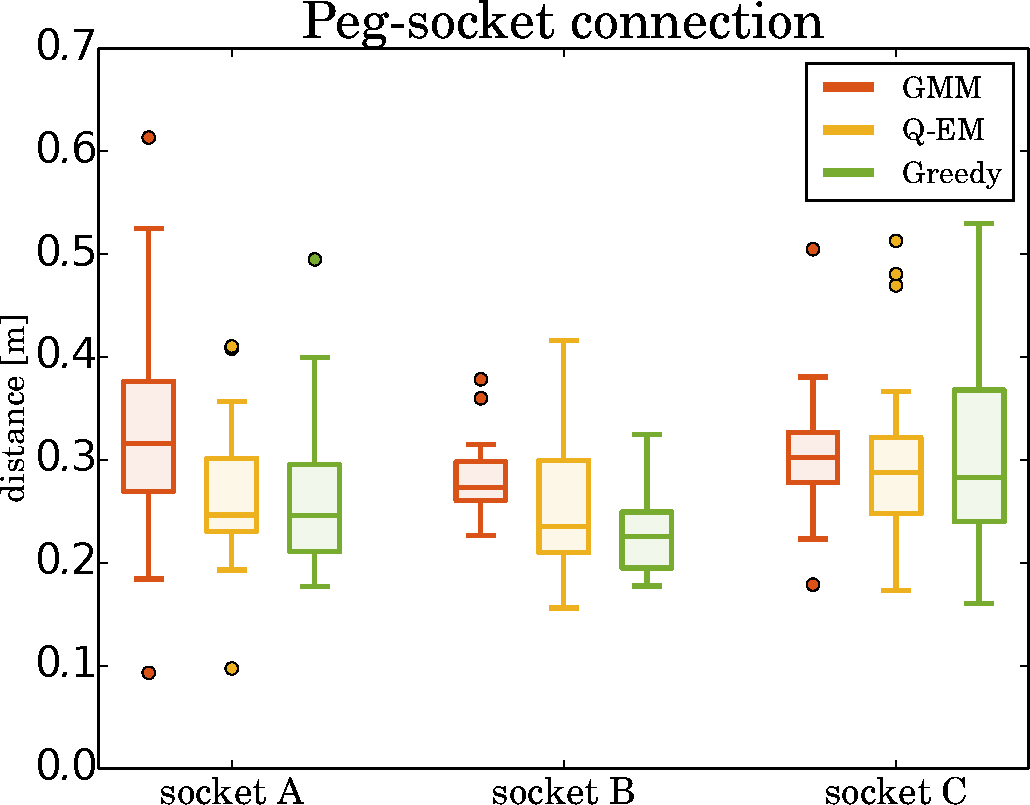
\includegraphics[width=0.9\linewidth]{./Figures/Results2/peg_socket_connection_v2.pdf}
  \caption{Distance taken (measured from point of contact of plug with socket edge) to connect the plug to the socket.}
  \label{fig:real_statistics2}
\end{figure}


Figure \ref{fig:real_statistics2} illustrates the statistics of the distance taken to establish a connection for all three sockets. 
The interesting point is that both the GMM and Q-EM algorithms perform better than the Greedy approach for socket C. Socket C has no informative 
features on its surface and as a result myopic policies such as the Greedy policy will perform poorly. However for socket A 
and B, the Greedy policy performs better as both of these sockets have edges around their connector point allowing for easy localisation. 
It can also be seen that most search methods perform better on socket B than A, since the funnel shape connector helps in maintaining the plug 
within the vicinity of the socket's holes. 


The discrepancy between the humans performance and the search policies can be attributed to many causes. One plausible reason is 
that the PMF probability density representation of the belief is more accurate than the human teachers position belief. 
Also, the motion noise parameter was fixed to be proportional to the velocity and the robot moves at gentle pace ($\sim1$ cm/s) as 
opposed to some of the human teachers. In actuality, humans are far less precise than the KUKA which has sub-millimetre accuracy.

\section{Discussion \& Conclusion}\label{sec:conclusion}
% Recapulate what we did 

In this work we learned search policies from demonstrations provided by human teachers for a task
which consisted of first localising a power socket (either socket A, B or C) and then connecting it with a plug. Only haptic information 
was available as the teachers were blindfolded. We made the assumption that the position belief of the human teachers 
was initially uniformly distributed in a fixed rectangular region of which they were 
informed and is considered prior knowledge. All subsequent beliefs were then updated in a Bayesian recursion 
using the measured velocity obtained from a vision tracking system, and wrench acquired from a force torque sensor attached 
to the plug. The filtered probability density function, represented by a Point Mass Filter, was then compressed to the 
most likely state and entropy.

Two Gaussian Mixture Model policies were learned from the data recorded during the human teachers' demonstrations. 
The first policy, called Q-EM, was learned in an Actor-Critic RL framework in which a value function was learned over 
the belief space. This was then used to weight training datapoints in the M-step update of Expectation-Maximisation (EM). The second 
policy, called GMM, was learned using the standard EM algorithm, and considered all training data points equally,
following in the footsteps of our initial approach \cite{Chambrier2014}. Both the Q-EM and GMM policies were trained 
with data solely from the demonstrations of the search with socket A.

We evaluated 4 different aspects of the learned policies. Firstly, we evaluated which of three policies, Q-EM, GMM and a Greedy policy, 
took the least distance to find the socket. We concluded that across three different Experiments the Q-EM algorithm always performed
the best. It was clear that the Q-EM policy was less random and more consistent than the GMM policy as it tried to enter in 
contact with the wall at the same height as the socket thus increasing the chances of finding the socket.

Secondly, we tested the importance of the data provided by the human teachers. We took the worst two teachers and trained an
individual GMM and Q-EM policy for each of them. We found that the performance of the Q-EM was better than the GMM in terms 
of distance travelled to find the socket. When qualitatively evaluating the trajectories of the GMM with respect to the 
Q-EM for the worst teacher, it is clear that the Q-EM policy managed to extract a search pattern, which was not the case 
for the GMM policy. We also tried to learn a Q-EM policy from the data provided by a Greedy policy with explorative noise 
and we found no improvement. From these results we conclude that the exploration and exploitation aspects of the trajectories 
provided by the human teachers is necessary.

Thirdly, we tested whether the two policies (GMM and Q-EM) were able to generalise to a different socket location. Under a specific condition,
which we called \textit{Fixed}, both policies were significantly better than the Greedy policy. However for the \textit{Center}
and \textit{Left} initial conditions the Greedy policy performed better. For the initial conditions in which the Greedy policy 
enters in contact with the wall at an early stage, it also performs better than the GMM and Q-EM. The reason for this is that  
the actions taken by the Greedy policy in this setting will always result in a decrease of entropy when the location
of the socket is close to a corner, as opposed to being in the center of the wall.

Fourthly, we evaluated all three policies on the KUKA LWR4 robot and found that all the policies did better than the human 
teachers. For socket A, on which both the GMM and Q-EM policies were trained, there is no clear distinction between 
the Q-EM and Greedy policy. On socket B, which was novel, the Greedy policy performed better than the statistical controllers, 
which we hypothesize was a result of a funnel which would make it easier for a myopic policy. For socket C, both the 
GMM and Q-EM policies performed better than the Greedy, as socket C has no features on its surface, this being a disadvantage 
for a myopic policy.

We conclude by making the observation that by simply adding a binary reward function in combination with 
data provided by human demonstrations, with Fitted reinforcement learning, we can learn a better policy without 
the need to perform expensive exploration-exploitation rollouts traditionally associated with reinforcement learning and 
designing complicated reward functions. This is especially advantageous when only a few demonstrations are available.


\appendix


\bibliographystyle{elsarticle-harv} 
\bibliography{bib/peg_hole.bib,bib/pomdp.bib,bib/RL.bib,ch3-citations.bib,bib/DT.bib,bib/MLMF.bib,bib/spatial_navigation.bib}

\end{document}

\endinput
%%
%% End of file `elsarticle-template-harv.tex'.